\newacronym{cem}{CEM}{Computational Electromagnetics}
\newacronym{em}{EM}{Electro Magnetic}
\newacronym{abc}{ABC}{Absorbing Boundary Conditions}
\newacronym{fdtd}{FDTD}{Finite-Difference Time-Domain}
\newacronym{pml}{PML}{Perfectly Matched Layer}
\newacronym{fa}{FA}{Finite Automaton}
\newacronym{dfa}{DFA}{Deterministic Finite Automaton}
\newacronym{nfa}{NFA}{Nondeterministic Finite Automaton}
\newacronym{fsm}{FSM}{Finite State Machine}
\newacronym{bnf}{BNF}{Backus-Naur form}
\newacronym{ebnf}{EBNF}{Extended Backus-Naur form}
\newacronym{abnf}{ABNF}{Augmented Backus-Naur form}
\newacronym{wsn}{WSN}{Wirth Syntax Notation}
\newacronym{peg}{PEG}{Parsing Expression Grammar}
\newacronym{asdl}{ASDL}{Zephyr Abstract Syntax Definition Language}
\newacronym{cfg}{CFG}{Context Free Grammar}
\newacronym{ast}{AST}{Abstract Syntax Tree}
\newacronym{ll}{LL}{Left-to-Right, Leftmost Derivation}
\newacronym{lalr}{LALR}{Look-Ahead, Left-to-Right, Rightmost Derivation}
\newacronym{glr}{GLR}{Generalized Left-to-Right Rightmost Derivation}
\newacronym{1d}{1D}{One Dimension}
\newacronym{2d}{2D}{Two Dimensions}
\newacronym{3d}{3D}{Three Dimensions}
\newacronym{cfl}{CFL}{Courant-Friedrichs-Lewy}
\newacronym{lumex}{LUMEX}{Lumerical Meep Exchange}
\newacronym{mpi}{MPI}{Message Passing Interface}
\newacronym{lhs}{LHS}{Left-Hand Side}
\newacronym{rhs}{RHS}{Right-Hand Side}




\chapter{Note to the Reader}
The following notation conventions apply throughout the thesis if not explicitly stated otherwise.  In the context pertaining to physics, symbols in \textbf{bold} represent vectors and symbols in \emph{italics} represent scalars, unless stated differently.
The del operator denoted by the nabla symbol $\nabla$ is used with the dot product and cross product to denote divergence: $\nabla \cdot v$ and the curl: $\nabla \times v$.
The expression "iff" refers to "if and only if".
In the context of regular languages, lower case Latin alphabet letters, such as $a, b, c, \dots$, refer to terminal symbols. Upper case Latin alphabet letters, such as $A, B, C,\dots$, denote nonterminal symbols.

Otherwise fairly standard notation in the applicable fields is used throughout the rest of the thesis. 

\chapter{Introduction}
In modern society, humans are reliant on a multitude of technologies, such as the Internet, mobile phones, television, radio, microwave ovens, camera sensors, lasers, light-emitting diodes, electrical motors, medical imaging systems, and many others. All of these rely on electromagnetic devices; electromagnetism undoubtedly plays a key role in day-to-day life as we know it.


The electromagnetic field theory is the underpinning framework for studying the effects of electromagnetic phenomena at scales where quantum effects are negligible. It studies the interactions between electric charges and currents (Currents are often referred to as electric charges in motion). Maxwell's equations are a series of fundamental coupled partial differential equations that form the cornerstone of classical electromagnetism. However, the closed-form analytical solutions are highly complex and available only for simple cases, making them impractical for most real-world applications.


However, with the rapid increase of available computational power, the use of analytically simple but computationally taxing methods was given an extra boost as they became more available. Compared to their counterparts, these methods provide solutions to more general problems. The branch of electromagnetics that focuses on such methods is termed \gls{cem}. \gls{cem} allows us to simulate more complex problems and verify designs before the production of prototypes. They also provide key insight into the operation of electromagnetic devices and even reveal certain information that may be unattainable by classical analytical methods. Moreover, with the ability to tweak the parameters and re-simulate, \gls{cem} has caused the advent of design optimization in electromagnetic devices.

\todo{motivation for use in company}
\todo{-> use mainly for 3d pohotonics, focus on that}
Today, many such tools and software packages exist, some commercial and others open-source. It is important to be able to verify the results against other implementations, which allows the researchers to verify whether the results are mere artifacts of a particular solver or physically meaningful. Furthermore, the tools may offer different features and constraints, and their interoperability is desired. 

This thesis explores the possibility of translating simulation code between two such tools, Ansys Lumerical\copyright and Meep. To address these challenges, this thesis develops \gls{lumex}, a tool that provides a framework for the translation of Lumerical Scripting Language to Meep.



  
  

\chapter{Review of Relevant Concepts}
This chapter aims to give the reader a broader understanding of the relevant subject matter. It provides an overview of the physics behind the aforementioned simulations and an introduction to the basic concepts of compiler design and the underlying formal language theory. This chapter will not delve into the specifics of each subject at hand but will rather provide the reader with the foundations necessary to comprehend the remaining parts of this thesis.

\section{Computational Electromagnetics}
As this thesis focuses on the implementation of a transpiler, an intricate grasp of \gls{cem} is not required; however, a surface-level explanation may benefit the reader, and thus it is provided below.

As explained earlier, \gls{cem} is a branch of electromagnetics that focuses on computational methods. This process involves modeling the interactions of \gls{em} fields with objects, typically with the computation of the $\mathbf{E}$ (electric) and $\mathbf{H}$ (magnetic) fields or the surface current, in the case of Method of Moments, across the simulation domain. These methods discretize the fields in a step called \emph{meshing}, resulting in the subdivision of the problem domain into many smaller elements. Depending on the simulation method and number of dimensions, this may result in a three-dimensional grid, two-dimensional patches or one-dimensional segments. There are multiple different methods, that each have specific use cases, Finite Element Method is useful when facing arbitrary geometry or objects that do not align properly in the Cartesian grid. Method of Moments is a surface-based method that converts integral forms of Maxwell's equations into matrix equations. \gls{fdtd} solves Maxwell's equations in the time domain and it is one of the most commonly used methods and also a key part of this thesis, so it will be introduced in more detail in the following sections~\cite{davidson_2010}.


\begin{figure}[H]\label{fig:double-slit}
  \centering
  \includegraphics[width=0.75\textwidth]{obrazky-figures/double-slit.pdf}
  \caption{Visualization of the electrical field in the famous double slit experiment.}
\end{figure}




\subsection*{Curl theorem}
\todo{ask if should omit}
\subsection*{Divergence theorem}
\todo{ask if should omit}
\subsection*{Maxwell's equations}

In the 19th century, James Clerk Maxwell formulated a set of four equations that underpin classical electromagnetic and form a coherent theoretical structure. 
Maxwell's equations in the integral form tend to be used in the calculation of symmetric problems, such as finding the electric field of a charged plane, sphere, etc., whereas the differential form is more suitable for the calculation of numerical problems as it is simple to obtain the magnetic and electric fields at a single point. The Ampère-Maxwell law states that magnetic fields are generated by electric currents and a change of the electric field over time. Faraday's law states that a changing magnetic field produces a rotating electric field and the other way around. Gauss's law for electric flux states that electric charges generate an electric field. Gauss's law for magnetic flux postulates the nonexistence of magnetic charge, i.e., magnetic monopoles. In 1931, Dirac proposed that the discovery of magnetic charge (a magnetic monopole) would require a modification of Gauss's law for magnetic flux~\cite{dirac1931monopole}. \todo{ask if this citation is OK} Despite extensive searches, magnetic monopoles have yet to be detected experimentally. 


Ampère-Maxwell law
\begin{equation}
\nabla \times \mathbf{H} =\mathbf{J} + \frac{\partial \mathbf{D}}{\partial t}
%\nabla \times \mathbf{B} =\mu_0\mathbf{J} + \mu_0 \epsilon_0 \frac{\partial \mathbf{D}}{\partial t}
\end{equation}

Faraday's law
\begin{equation}
\nabla \times \mathbf{E} = - \frac{\partial \mathbf{B}}{\partial t}
%\nabla \times \mathbf{E} = - \frac{\partial \mathbf{B}}{\partial t}
\end{equation}

Gauss's law for electric flux
\begin{equation}
\nabla \cdot \mathbf{D} = \rho
%\nabla \cdot \mathbf{E} = \frac{\rho}{\epsilon_0}
\end{equation}

Gauss's law for magnetic flux
\begin{equation}
\nabla \cdot \mathbf{B} = 0
\end{equation}

%= 4\pi\cdot 10^{-7} \si{\volt\second}/\si{\ampere\meter}


%Where $\mathbf{B}$ is the magnetic field, $\mathbf{E}$ is the electric field, $\mathbf{J}$ the current density, $\mu_0$ the vacuum permeability, $\epsilon_0 = $ the vacuum permittivity. It also holds that the speed of light $c=\left(\epsilon_0\mu_0\right)^{-\frac{1}{2}}$.

The above equations are in the differential form, and they are first-order linearly coupled. They also have equivalent integral forms, which may be produced by applying the divergence integral theorem and curl integral theorem. Readers are directed to~\cite[Chapter~2.4]{staelin2009electromagnetics} for more details. \todo{ask if okay}




\subsubsection*{Constitutive Relations}
Since Maxwell's equations contain more unknowns than equations, as shown above, they are undetermined. This is where constitutive relations between field intensities $\mathbf{E},\mathbf{H}$ and the flux densities $\mathbf{D},\mathbf{B}$ come into play. 
For simple mediums, which are \emph{linear}, \emph{isotropic}, and \emph{non-dispersive}, the following equations hold.


\begin{equation}
\mathbf{D} = \epsilon \mathbf{E}
\end{equation}
\begin{equation}
\mathbf{B} = \mu \mathbf{H}
\end{equation}
\begin{equation}
\mathbf{J} = \sigma \mathbf{E}
\end{equation}

Where $\epsilon$, the permittivity of a medium, is given by the permittivity of free space and the relative permittivity respectively $\epsilon = \epsilon_0\epsilon_r$. Similarly, $\mu$, the permeability of a medium, is given by the permeability of free space and the relative permeability $\mu = \mu_0\mu_r$. A medium is often defined by its \emph{constitutive parameters} $\epsilon$, $\mu$, $\sigma$. A good illustration of this is that a medium is \emph{isotropic} if $\epsilon$ does not change with direction, \emph{homogeneous} if $\epsilon$ does not change between two different points in space. Another example is that a material is \emph{linear} if $\mathbf{D} = \epsilon \mathbf{E}$ holds and $\epsilon$ does not change in respect to $\mathbf{E}$.





\subsection*{Finite Difference Time Domain}
The \gls{fdtd} method is a staple among finite difference techniques. Finite difference methods are numerical techniques that approximate derivatives directly using finite difference quotients. This class of methods is widespread due to its implied simplicity and is widely used for scientific computation. 


It is suitable for problems where the electromagnetic wavelengths, along with the geometries, are comparable to the simulation domain. It is a time domain method, thus it may solve for a broad spectrum in a single simulation in a single pass where it provides a direct numerical approximation of the differential operators in Maxwell's curl equations. The spatial domain is discretized into a staggered grid of \emph{cells}; these will be explained in more depth soon. \gls{fdtd} also discretizes the continuous time into \emph{time steps}, how-ever there is a limit to the largest time step, where the method stays numerically stable, $\Delta t < h / \left( c \sqrt{3} \right)$ for \gls{3d}, where $h$ and $c$ denote the grid dimension and speed of light in the simulation respectively. This is often referred to as the \emph{Courant limit} after the \gls{cfl} condition.


The user must keep in mind that such a method will never give a precise answer. The accuracy of the simulation is dictated by the resolution. A general rule of thumb in the \gls{cem} community is to use at least 10 samples (cells) per the shortest wavelength. Similarly, Dennis M. Sullivan's book Electromagnetic Simulation Using the FDTD Method states: “A good rule of thumb is 10 points per wavelength. Experience has shown this to be adequate, with inaccuracies appearing as soon as the sampling drops below this rate.”~\cite[p.10]{sullivan2013fdtd}.\todo{ask if this citation is OK}


\gls{fdtd} provides second-order accuracy with the use of first-order numerical differentiation. Thus the error may be defined as $\text{Error} \propto (\Delta h)^2$. For example, in a \gls{3d} simulation, if the spatial (and thus time) resolution is increased twofold, the accuracy increases 4 times. This is due to the fact Maxwell’s curl equations are discretized using central difference approximations, which are inherently second-order accurate.


Another vital part is the staggered grid it self. Kane S. Yee introduced a system of calculating the $\mathbf{E}$ and $\mathbf{H}$ fields using the aforementioned central differences in an offset pair of grids. The $\mathbf{E}$ fields are defined at the edges of a cell while the $\mathbf{H}$ fields are stored at the centers of the faces, thus offset spatially by $\frac{h}{2}$.  However since the $\mathbf{E}$ and $\mathbf{H}$ fields are defined at different locations, the time step must be staggered as well. The $\mathbf{E}$ field is calculated at time $t$ and the $\mathbf{H}$ field at $t + \frac{\Delta t}{2}$. This is known as the Yee cell, and it is a cornerstone of \gls{fdtd} methods. The Yee cell is shown in \cref{fig:yee}.


\begin{figure}[H]\label{fig:yee}
  \centering
  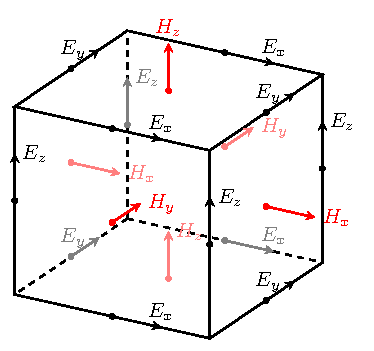
\includegraphics[width=0.75\textwidth]{figures/yee.pdf}
  \caption{Description of the Yee cell.}
\end{figure}

The basic flow of the \gls{fdtd} algorithm is as follows:
\begin{enumerate}
\item Divide the solution region into a grid of nodes (the Yee cell grid).
\item Approximate the derivatives in Maxwell's equations using finite differences at these nodes.
\item Set the initial conditions for the electric and magnetic fields.
\item Loop over time steps using the "leapfrogging" technique:
\begin{enumerate}
  \item Update the electric field components using values of the magnetic field from the previous half time step.
  \item Update the magnetic field components using the newly computed values of the electric field.
\end{enumerate}
\item Apply boundary conditions during each time step.
\item Store the field values at desired time points for later analysis.
\item Continue time marching until the desired simulation time is reached.
\end{enumerate}



\subsection{Boundary Conditions}
\todo{this}

\section{Meep}
Meep --- MIT Electromagnetic Equation Propagation --- is an open-source program for \gls{em} simulations distributed under the GNU General Public License v2.0. It is a scriptable software package using Python, Scheme or C++ APIs, however it lacks a graphical user interface. Nonetheless this allows the combination of multiple computation and a multi-parameter optimization, even in parallel. Meep handles paralelization across multiple cores and systems using the \gls{mpi}\footnote{\url{https://www.mpi-forum.org/}}. 

Meep allows simulating in \gls{1d}, \gls{2d}, \gls{3d} and cylindrical coordinates. It can handle arbitrary geometries and materials such as anisotropic, dispersive, nonlinear and gyrotropic materials. It also supports a variety of boundary conditions, including Bloch-periodic, perfect-conductor boundary conditions and perfectly matched layers. 

Meep offers the ability to exploit symmetries to reduce the computational time and memory requirements. The $\mathbf{E}$ and $\mathbf{H}$ fields may be exported and loaded using the HDF5 file format. These may be converted to other formats, such as VTK and visualized using ParaView\footnote{\url{https://www.paraview.org/}}. 
\todo{expand}

\section{Ansys Lumerical}
Ansys Lumerical FDTD\copyright \ is a photonics simulation tool that combines \gls{fdtd}, Optical Multilayer Solvers, Rigorously Coupled-Wave Analysis Solvers, Waveguide Solvers, Finite-difference Eingenmode Solvers and others within a unified design environment\footnote{Any and all ANSYS, Inc. brand, product, service and feature names, logos and slogans such as Ansys Lumerical are registered trademarks or trademarks of ANSYS, Inc. or its subsidiaries in the United States or other countries. All other brand, product, service and feature names or trademarks are the property of their respective owners.}.
\todo{expand}


\section{Formal Language Theory}
We use languages like English, Czech, or Slovak in everyday communication exchanges, and these languages are commonly referred to as \emph{natural languages}. The Oxford English Dictionary defines language as a system of spoken or written communication used by a particular country, people or community. How-ever, a more rigorous definition of languages and the tools to operate within them is required. These aspects of language will be tackled in the notion of formal language, which is introduced in the below sections.

\subsection{Alphabets and Languages}

\todo{add text about languages and alphabets, use English as example}
Languages, both natural and formal, are constructed from a basic set of elements. In the case of English, these elements are the letters A to Z, which form the English alphabet. From this alphabet, we can produce words, which in turn form sentences and larger linguistic structures. Similarly, in formal language theory, we start with an alphabet from which we build sequences known as words. These words serve as the foundational units of formal languages, just as words do in natural languages.

\begin{definition}[Alphabet]\label{def:alphabet}
Let $\Sigma$ be an \emph{alphabet}, a finite nonempty set of symbols, letters. Then $\Sigma ^{*}$ defines the set of all sequences $w$:
$$w= a_1 a_2 a_3 \dots a_{n-1} a_n, \in \Sigma \text{ for } n \in \mathbb{N}$$
\end{definition}

The sequence of symbols $w$ is called a \emph{word}. Word length is given by the number of symbols $a$, and symbolically annotated as $|w| = n$. The word with a length of 0 is called an \emph{empty word} denoted as $\epsilon$.

\begin{definition}[Language]\label{def:language}
The set $L$ where $L\subseteq \Sigma^{*}$ is defined as a \emph{formal language} over the alphabet $\Sigma$. 
\end{definition}
The words $L = \left\lbrace \epsilon, a, b, aa, ab, bb \right\rbrace$ are examples of words in language $L$ over the alphabet $\Sigma=\left\lbrace a,b \right\rbrace$.
Other examples of languages over the alphabet $\Sigma=\left\lbrace a,b \right\rbrace$ might include:
\begin{itemize}
\item $L_1 = \left\lbrace \epsilon \right\rbrace$
\item $L_2 = \left\lbrace a \right\rbrace$
\item $L_3 = \left\lbrace aaa \right\rbrace$
\item $L_4 = \left\lbrace a^i,b^i; i \in \mathbb{N} \right\rbrace$
\end{itemize}




\paragraph*{Notation conventions}



\begin{itemize}
\item Iteration\\
  Let $a^i; a \in \Sigma \text{ and } i \in \mathbb{Z}$ be the \emph{iteration} of a character $a$, where $|a^i| = i$.\\
Examples bellow:


\begin{itemize}
\item $a^0 = \epsilon$
\item $a^1 = a$
\item $a^2 = aa$
\item $a^i = a_0 a_1 a_2 \dots a_i; i \in \mathbb{N}$
\end{itemize}


\item Concatenation\\
  Let $w \cdot w^{'}; w, w^{'} \in \Sigma^{*}$ be the \emph{concatenation} of the words $w$ and $w^{'}$.

$w = a_1 a_2 a_3 \dots a_n ; w^{'} = a^{'}_1 a^{'}_2 a^{'}_3 \dots a^{'}_m; n,m \in \mathbb{Z}$ then  

$w\cdot w^{'} = w w^{'} = a_1 a_2 a_3 \dots a_n a^{'}_1 a^{'}_2 a^{'}_3 \dots a^{'}_m$


\item Kleene star\\
  Let $L \subseteq \Sigma^{*}$ be a language. The \emph{Kleene star} of $L$, denoted $L^{*}$, is defined as
  \[
    L^{*} \;=\; \bigcup_{i=0}^{\infty} L^{i},
  \]
  where $L^{0} = \{\epsilon\}$ and $L^{i+1} = L \cdot L^{i}$.  Equivalently, $L^{*}$ is the set of all finite concatenations of zero or more words from $L$.\\

\item Symbol count\\
The number of occurrences of $a$ in $w$, where $a \in \Sigma, w \in \Sigma^{*}$, noted as $|w|_{a}$.

\end{itemize}

\subsection{Grammars}
Linguists refer to grammar as a set of surface level and deep level rules that specify how a natural language is formed. Due to the polysemous and homonymous nature of natural languages, it is not suited for the description of unambiguous systems. The inherit need to strictly describe languages introduced various language defining mechanisms. Many of these mechanisms are interchangeable, and may describe the same languages. However, not all mechanisms are able to describe languages formed by other mechanisms.

The concept of a grammar is a powerful tool for describing languages~\cite[p. 52]{Linz2016Introduction}. A simple sentence in English consists of a single independent clause. A clause is typically formed by a subject and a predicate. This can be written as follows.
$$ \left< clause \right> \rightarrow \left< subject \right> \left< predicate \right> $$

We can further define the $\left< subject \right>$ and $\left< predicate \right>$. One of the possible subjects is a noun phrase, and the predicate may be a simple verb.
$$\left< subject \right>   \rightarrow   \left< determiner \right>   \left< premodifier \right>    \left< noun \right>    \left< postmodifier \right>$$
$$\left< predicate \right> \rightarrow \left< verb \right>$$

Associating the $\left< determiner \right>$ with the article "the", $\left< premodifier \right>$ with "fast" or "slow", $\left< noun \right>$ with "athlete", $\left< postmodifier \right>$ to "from England" or to an empty string and finally associating the $\left< verb \right>$ to "won" or "lost" allows us to define a pattern capable of generating an infinite number of clauses/sentences such as "The fast athlete from England won" or "The slow athlete lost", which testifies to the principle of Chomskian generative grammar.. These sentences are considered to be \emph{well formed} as far as grammar is concerned, as they resulted from the implementation of grammatical rules.

The premise is to consecutively replace the $\left< clause \right>$ until only irreducible blocks of the language remain. Generalizing this idea brings about the concept of formal grammars.

\begin{definition}[Grammar]
\label{def:grammar}
Let an ordered quadruple $G$ define a grammar such that: $G=\left(N, \Sigma, P, S \right)$, where~\cite{Salomaa1987Formal}:
\begin{enumerate}
\item $N$ is a finite set of \emph{nonternminal} symbols
\item $\Sigma$ is an alphabet, i.e. a finite set of \emph{terminal} symbols, such that $N \cap \Sigma = \varnothing$
\item $P$ is a finite set of rewriting rules known as \emph{productions}, ordered pairs $\left( \alpha, \beta \right)$.
$P$ is a subset of the cartesian product of $\alpha = \left(N \cup \Sigma\right)^* N \left(N \cup \Sigma\right)^*$ and $\beta = \left(N \cup \Sigma\right)^*$


The productions are denoted as $\alpha \rightarrow \beta$.
If there are multiple productions with the same left hand side ($\alpha$), we can group their right hand sides ($\beta$).


$\alpha \rightarrow \beta_1, \alpha \rightarrow \beta_2$ may be written as $\alpha \rightarrow \beta_1 | \beta_2$

\item $S$ is the starting symbol of the grammar $G$, where $S \in N$
\end{enumerate}
\end{definition}

Productions $\alpha \rightarrow \beta$ symbolize, that given the words $V,W,x,y \in \left( N \cup \Sigma \right)^{*}$, the word $V$ can be rewritten as follows:
$V \Rightarrow W$ iff there are words, which satisfy the following condition, $V=x\alpha y \wedge W=x\beta y$ and $\alpha \rightarrow \beta \in P$.

\begin{definition}[Derivation]
\label{def:derivation}
$V \stackrel{*}{\Rightarrow}  W$ iff there is a finite set of words 
$$ v_0, v_1, v_2, \dots, v_z;\medskip z \in \mathbb{Z}$$
such that $v_0 = V$ and $v_z = W$ where each is rewritten from the previous word. Such a sequence of applications of productions is called a derivation.
The length of a derivation is given by $z$. 
\end{definition}

Grammars are often represented using formalisms that, often set restrictions on the left and right hand sides of productions. These restrictions further impose limits on the set of languages a grammar may produce; this is known as the \emph{expressive power} of a grammar. 

\subsection{Chomsky hierarchy}
When working with formal grammars, the need to compare their expressive power arose. Linguist Noam Chomsky introduced the so called \emph{Chomsky hierarchy}~\cite{chomsky1956three}. A set of four classes, each more expressive than the previous, see \cref{fig:chomsky-hierarchy}.



\begin{figure}[H]\label{fig:chomsky-hierarchy}
  \centering
  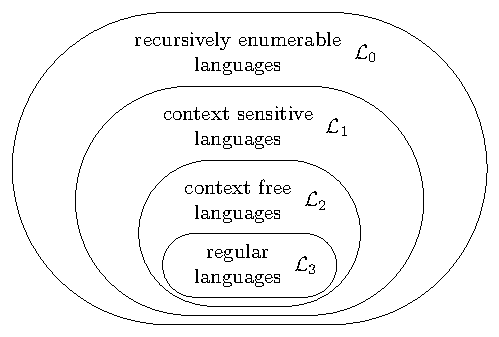
\includegraphics[width=0.75\textwidth]{figures/chomsky-hierarchy.pdf}
  \caption{Description of the Chomsky hierarchy.}
\end{figure}

The intricacies of each of said classes are not necessary in the context of this thesis, how-ever regular and context free languages will be used heavily throughout the rest of this thesis, and explained more in depth.

\begin{table}[h]\label{tab:chomsky-hierarchy}
\centering
\begin{tabular}{|ccl|}
\hline
Grammar         & Language               & Restrictions \\ 
\hline
$\mathcal{L}_3$ & Regular                & \todo{todo}             \\
\hline
$\mathcal{L}_2$ & Context Free           &              \\
\hline
$\mathcal{L}_1$ & Context Sensitive      &              \\
\hline
$\mathcal{L}_0$ & Recursively Enumerable &              \\ 
\hline
\end{tabular}
\caption{An overview of the Chomsky hierarchy classes.}
\end{table}


\subsection{Regular Languages}
As shown above, regular languages are the inner most part of the Chomsky hierarchy, thus they are the most constricted. How-ever, regular languages play a crucial role in lexical analysis, more precisely, in pattern matching. These constrictions lead to many useful closure properties and decisability properties, mainly membership, which will be introduced shortly.

Regular languges may be defined in multiple equivalent manners such as through finite automata or regular expressions. 

\subsubsection{Finite Automata}

\begin{definition}[Deterministic Finite Automata]\label{def:dfa}
\glspl{dfa} are formally defined as 5-tuples
$$ M = (Q, \Sigma, \delta, q_0, F),$$ 
where
\begin{itemize}
\item $Q$ is a finite set of states,
\item $\Sigma$ is a finite set of symbols, also known as an input alphabet,
\item $\delta$ is a transition function between states defined as $\delta : Q \times \Sigma \rightarrow Q$,
\item $q_0$ is a initial state for which $q_0 \in Q$ holds true,
\item $F$ is a set of final states, $F \subseteq Q$.
\end{itemize}


If starting in the state $q_0$ and moving left to right over the input string such that during each move a single symbol is consumed from the input string and a transition function for the corresponding state and symbol exists, and all symbols from the input string have been read and the \gls{dfa} stopped in a final state, the string is deemed accepted. This is called a deterministic finite acceptor.
\end{definition}

Similarly \glspl{nfa} ale a 5-tuple, however they may have multiple initial and final states and there may be multiple transitions from the same state using the same symbol. For a rigorous formal definition the reader is directed to~\cite[Chapter~1.4]{Salomaa1987Formal}.

\begin{figure}[H]\label{fig:dfa}
  \centering
  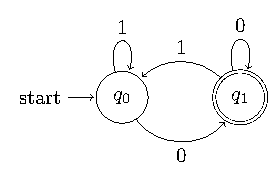
\includegraphics[width=0.5\textwidth]{figures/dfa.pdf}
  \caption{A \gls{dfa} accepting only even binary numbers.}
\end{figure}

An example of a \gls{dfa} that accepts only even binary numbers is provided above. For a binary number to be even, the least significant bit must be a $0$. When this \gls{dfa} consumes a $1$, it stays or returns to the initial non-accepting state $q_0$, when it consumes a $0$, beaning the current least significant bit is $0$, is moves to an accepting state $q_1$. Leading zeros are ignored.





\subsubsection{Regular Expressions} 

\begin{definition}[Regular Expressions]\label{def:regular_exp}
  Regular expressions are an algebraic notation, that describe a regular language. 
  
\begin{table}[ht]
\centering
\begin{tabular}{|ccc|}
\hline
\makecell{\textbf{Regular}\\ \textbf{Expression}} & \textbf{Language} & \textbf{Description} \\ 
\hline
a                          & $\{\text{"a"}\}$          & \makecell{The set containing a single\\ character "a"} \\
\hline
$\epsilon$                  & $\{\text{""}\}$           & The set containing the empty string \\
\hline
s|t                         & $L(s) \cup L(t)$            & Strings from both languages, union \\
\hline
st                          & $\{vw \mid v \in L(s), w \in L(t)\}$ & \makecell{All strings formed by\\ concatenating any string from\\ the first language with any string\\ from the second language.} \\
\hline
$s^*$                         & $\{\text{""}\} \cup \{vw \mid v \in L(s), w \in L(s^*)\}$ & \makecell{All concatenations of zero \\ or more strings from $L(s)$} \\
\hline
\end{tabular}
\caption{Regular Expressions and Their Languages.}
\label{tab:regex}
\end{table}
\end{definition}

An example of a regular expression that accepts only even binary numbers is provided bellow. The expression matches any number of ones and zeros but must always end with a zero.

\begin{figure}[H]\label{fig:regex}
  \centering
  $L1=\{\text{"}0\text{"}\}, L2=\{\text{"}1\text{"}\}$ $(L1\mid L2)^* L1$
  \caption{A regular expression accepting only even binary numbers.}
\end{figure}

It holds true that \glspl{nfa}, \glspl{dfa} and regular expressions are closed under union, concatenation and Kleene star. They are in all intents and purposes equivalent and may be converted between each other as shown in \cref{fig:conversion}.

\begin{figure}[H]\label{fig:conversion}
  \centering
  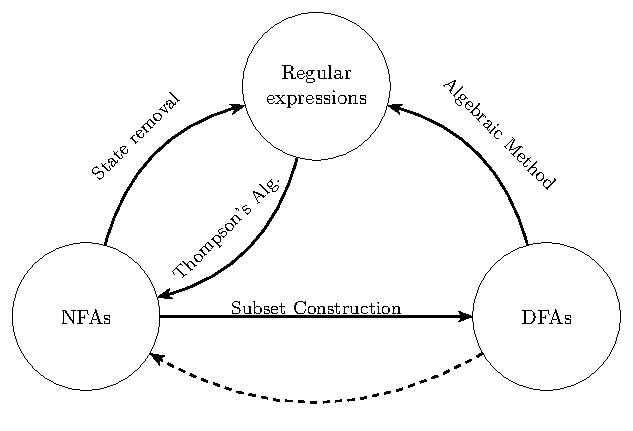
\includegraphics[width=0.75\textwidth]{figures/conversion.pdf}
  \caption{A diagram describing the equality of \glspl{dfa}, \glspl{nfa} and regular expressions.}
\end{figure}

Thus we have show that all 3 devices are equivalent and may be used to describe a $\mathcal{L}_3$ language.


\subsection{Context Free Languages} 

\subsubsection{LL Languages}



  


\section{Compilers}


Today's world relies on software more than ever before. It is imperative for developers to be able to write software efficiently. Software today is written in programming languages, high-level human-readable notations for defining how a program should run. However, before a program can be run on a system, it has to be translated (or compiled) into low-level machine code, which computers can run. The computer program that facilitates this translation is called a \emph{compiler}. See \cref{fig:compiler}.

\begin{figure}[H]\label{fig:compiler}
  \centering
  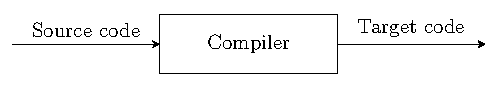
\includegraphics[width=0.75\textwidth]{figures/compiler.pdf}
  \caption{Description of a compiler as a single unit.}
\end{figure}



Compilers are complex programs. It is helpful to break them down into parts, each handling different tasks, which are chained together to form a compiler. Modern compilers are composed of many phases, such as the Lexical Analyzer, Syntax Analyzer, Semantic Analyzer, Intermediate Code Generator, Machine-Independent Code Optimizer, Code Generator, Machine-Dependent Code Optimizer~\cite[p. 5]{dragon}, however this chapter covers the components relevant to this thesis. See the relevant stages in \cref{fig:compiler-stages}.


\begin{figure}[H]\label{fig:compiler-stages}
  \centering
  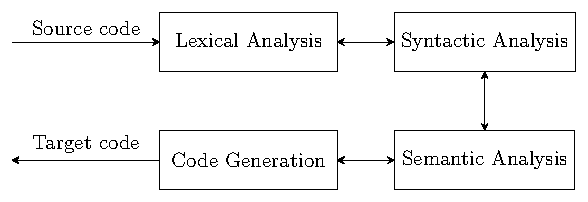
\includegraphics[width=0.75\textwidth]{figures/compiler-stages.pdf}
  \caption{Overview of relevant compiler stages.}
\end{figure}

\subsection*{Lexical Analysis}
The first stage of a compiler is lexical analysis, also known as a \emph{lexer} or \emph{tokenizer}. For the remainder of this thesis, the term \emph{lexer} will refer to the lexical analysis stage of a compiler. The lexer consumes a stream of characters, or the \emph{source code}, and returns a stream of \emph{tokens}. A \emph{token} is a lexically indivisible unit, for example, the Python keyword \texttt{return}, cannot be divided any further, e.g. into \texttt{re} \texttt{turn}. Each token is comprised of characters. The rule that defines which combination of characters constitutes a given token is called a \emph{pattern}. The sequence of characters matching a pattern is called a \emph{lexeme}, which is stored along with the token as a value.

%Lexical analysis may be further divided into two distinct stages, however they are often implemented together. These stages are the \emph{scanner} and \emph{evaluator}.


\subsubsection*{Regular Expressions}
\emph{Regular expressions}, which were introduced in \cref{def:regular_exp} are a compact way to represent the patterns accepting tokens. Regular expressions are an algebraic definition of patterns; they specify \emph{regular languages}, $\mathcal{L}_3$

\subsection*{Syntactic Analysis}

\subsubsection*{LL Parser}

\subsection*{Semantic Analysis}\label{sem-analysis}
\todo{talk about it being skipped and correct input code is relied on}

\subsection*{Code Generation}


\chapter{Transpiler Implementation}
This chapter introduces the implementation of the source to source compiler designed to convert Lumerical's scripting language to Python combined with the Meep library. 
\section{Choice of Tools}
When writing any program, it is important to choose the right tools for the job. This comes down not only to choosing the programming language but also what libraries and packages to utilize and which components to implement to better suit the project's constraints. The source language, Lumerical's scripting language, allows you to automate tasks and analysis such as manipulating simulation objects, launching simulations, and analyzing results~\cite{ansys_lsf}. This language how-ever, is not suitable for implementing a transpiler. Looking at the target language, Python is a general-purpose high-level interpreted language. Writing the transpiler in Python will allow for easier editing and debugging due to it's high-level nature. Consequently, and owing to the fact that the implementation language is the same as the target language, this will also allow us to use built in modules for generating the target code. Python's ecosystem also includes the tools such as Sphinx and Pytest for writing technical documentation and tests respectively.

\subsection{Implementation Overview}

The figure bellow describes the layout of the submitted work. \todo{make more verbose}

\begin{figure}[H]\label{fig:project-structure}
\centering
\dirtree{%
.1 /.
.2 doc/\DTcomment{Holds documentation.}.
.3 sphinx/\DTcomment{Sphinx root.}.
.4 build/\DTcomment{Sphinx build directory.}.
.5 html/\DTcomment{HTML output.}.
.4 source/\DTcomment{Sphinx documentation source.}.
.2 src/\DTcomment{LUMEX source code.}.
.3 actions.py\DTcomment{Code generation.}.
.3 grammar.py\DTcomment{Generic grammar class.}.
.3 lex.py\DTcomment{Lexer implementation.}.
.3 lltable.py\DTcomment{\gls{ll}$(1)$ parse table generator.}.
.3 lumerical\_grammar.py\DTcomment{Concrete instance of Grammar describing the Lumerical Scripting Language.}.
.3 lumex.py\DTcomment{Main script.}.
.3 parse.py\DTcomment{\gls{ll}$(1)$ table based parser implementation.}.
.3 runtime.py\DTcomment{Runtime code routines.}.
.3 symbol.py\DTcomment{Generic symbol class.}.
.3 tokens.py\DTcomment{List of tokens.}.
.2 tests/\DTcomment{Holds Pytest unit tests.}.
}

\caption{Overview of the project file structure.}
\end{figure}

\subsection{Sphinx}
Sphinx is a tool that automatically generates documentation by converting plain text source files into multiple output formats~\cite{sphinx_quickstart}. Sphinx was chosen because it facilitates the extraction of docstring style comments from the Python code, which may be enriched by the addition of ReStructured Text~\cite{docutils_rst}. Multiple output formats such as Portable Document Format, \LaTeX \ source code and Hypertext Markup Language, are supported. Sphinx also includes multiple extensions which allow the parsing of \LaTeX \ into Scalable Vector Graphics, which are easily rendered in the web.

This is instrumental in providing the user with the necessary insight into the technical operation of the transpiler, and allows us to search and view information in a concise manner withot the need to direcly inspect the source code. The documentation is made available to the reader at the following address \footnote{\url{https://www.macura.sk/LUMEX/}}.

\begin{figure}[H]

  \label{fig:shpinx}
  \centering
  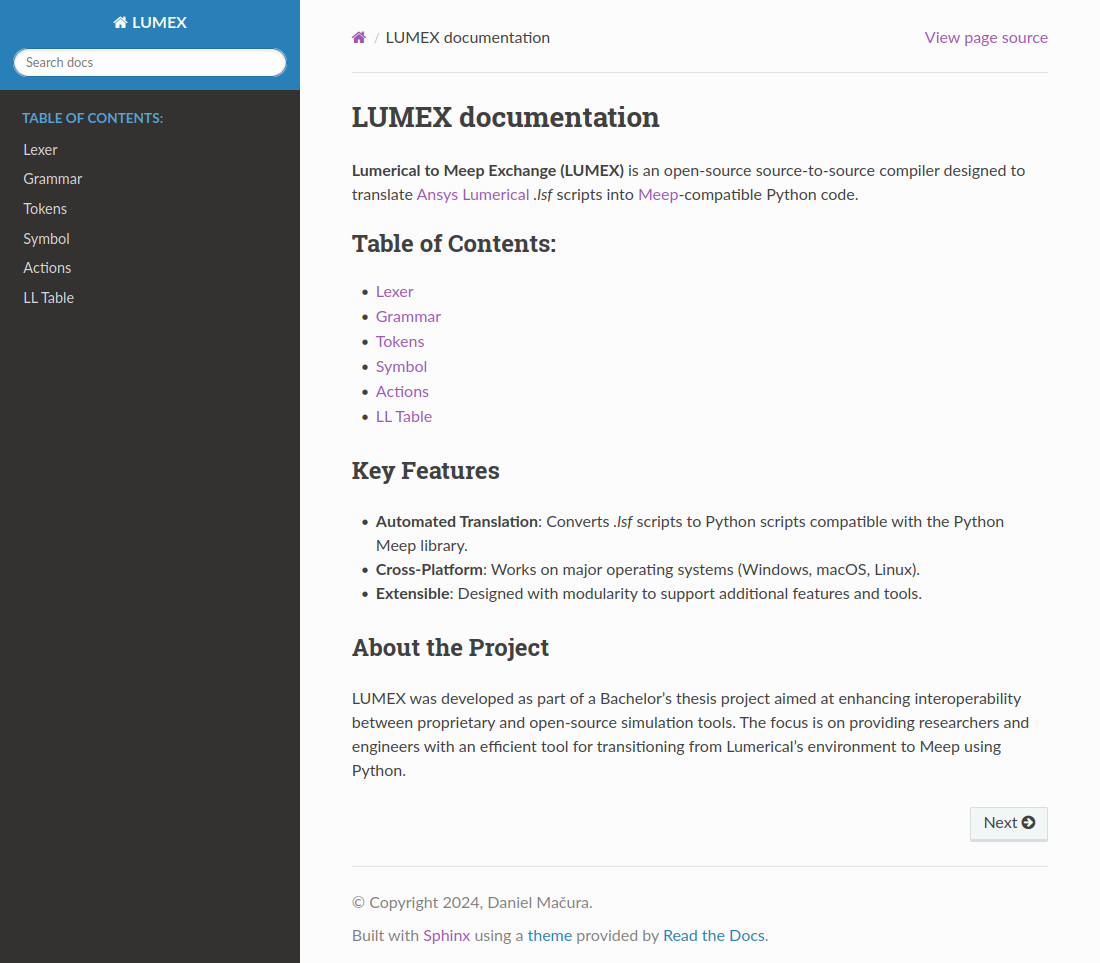
\includegraphics[width=\textwidth]{obrazky-figures/sphinx-lumex.png}
  \caption{Screen-capture of the resulting documentation.}
\end{figure}

\subsection{Pytest}
Pytest is a widely used testing framework for Python. 

%\section{General Implementation Strategy}
%The purpose of this thesis is to construct a custom transpiler between two highly specific languages, nevertheless it is beneficial to separate each logical step into its own class, which promotes interoperability and allows for simpler extension or replacement of code and parsing methods down the line. 

\todo{mention python, sphinx, pytest, explain motivation for implementation of own transpiler}



\section{Grammar}\label{grammar}
Before being able to translate between two languages, it is paramount to understand their grammar. Many languages provide definitions of grammars in a metasyntax format such as \gls{bnf}, \gls{ebnf}, \gls{wsn}, \gls{abnf}, \gls{peg} or \gls{asdl}~\cite{asdl}. The Python grammar is defined by a mixture of \gls{ebnf} and \gls{peg} as used in the CPython parser~\cite{python3grammar}. Additionally, the Python \gls{ast} module also defines an abstract grammar in \gls{asdl}~\cite{python_ast}.

As, of writing this thesis, Lumerical does not publicly provide any such specification for the Lumerical's scripting language. Thus, it is necessary to analyze the language and derive such a grammar that covers the relevant subset of the language to the scope of this thesis.

%To derive a grammar from a language, it is first necessary to specify the scope of the studied language.
Since this thesis focuses primarily on nanophotonic simulation workflows in \gls{3d}, only essential commands to set up a simulation will be included, e.g. commands to add blocks, sources, monitors and commands to translate and scale the objects. There may be other parts of Lumerical's scripting language that could be utilized for a nanophotonics simulation, however those are considered out of the scope of this thesis due to the broad range of Lumerical's scripting language with around 800 commands and keywords~\cite{ansys_lsf_commands}. Since Meep is a \gls{fdtd} solver, only commands usable in Lumerical \gls{fdtd} simulations will be considered.
While Lumerical’s scripting language includes hundreds of commands spanning optimization, analysis, and post-processing (e.g., \texttt{runoptimization}, \texttt{fitlorentzpdf}, \texttt{exportcsvresults}), this work prioritizes the core geometry and simulation workflow: \texttt{addrect} (block creation), \texttt{addplane}/\texttt{addfdtd} (source/solver definition), \texttt{addpower} (monitor placement), and \texttt{set} (property configuration). 


\todo{provide steps to reverse-engineer grammar}
There are infinitely many distinct grammars that describe the same language. By example, in a \gls{cfg} given as $S \rightarrow aB$, one may add an intermediate rule, producing $S \rightarrow aC, C \rightarrow B$. This process may be repeated indefinitely creating new grammars that describe the same language. To this end, the grammar described bellow is just one of the plethora of possible grammars describing a subset of Lumerical's scripting language. While constructing the grammar, it is beneficial to impose additional constrains and only utilize a subset of \glspl{cfg}, namely a \gls{ll} grammar. This imposes certain rules as described before, informally speaking, when a parser arrives at a nonterminal, is must be able to decide which production to apply by peeking at at most the next $k$ symbols, this is an \gls{ll}$(k)$ grammar.

This will later help with constructing a simpler parser. However if a language construct was found in Lumerical's scripting language, outside of the subset studied by this thesis, that could not be described and parsed by a \gls{ll}(1) parser or even a \gls{ll}(k) parser, a more powerful parser would be required. This would incur need to swap out the parser implementation in \texttt{parse.py}. Because of this and similar reasons, the transpiler was written in a modular fashion, making this a trivial matter. Other common parser types might include the \gls{lalr} parser which is stronger as the \gls{ll} parser but just as fast, or the \gls{glr} parser which can handle even more ambiguous grammars.


\todo{collecting samples}
It is important to first collect samples of code, to study the syntactic structure and the semantics of the code. Examples were taken from the official code 

Some examples are provided bellow that showcase the basic language constructs to the reader, a comprehensive list of commands is included in \cref{tab:commands} of Appendix~\ref{appendix:one}:

\paragraph*{Basic algebraic operators}
\begin{itemize}
\item \texttt{*} --- Multiplication
\item \texttt{\textbackslash} --- Division
\item \texttt{+} --- Addition
\item \texttt{-} --- Subtraction
\item \texttt{==} --- Comparison
\item \texttt{!=} --- Not equal
\item \texttt{<=} --- Less than or equal to
\item \texttt{>=} --- Greater than or equal to
\item \texttt{<} --- Less than
\item \texttt{>} --- Greater than
\item \texttt{:} --- Range
\begin{lstlisting}
1:2:10
\end{lstlisting}
Generates values 1, 3, 5, 7, 9.
\end{itemize}

Loops and conditionals
\begin{itemize}
\item \texttt{for} --- For loop
\begin{lstlisting}
for(1:10){ 
?x; 
} 
\end{lstlisting}

According to Ansys, ``There is no \texttt{while} command in the scripting language, but the \texttt{for} command can be used to implement a \texttt{while} command. The command \texttt{for(0; conditional\_expression; 0) \{\}} is the same as \texttt{while(conditional\_expression) \{\}}. The ``\texttt{0}'' statements in the \texttt{for} loop do nothing and are just placeholders because the scripting language expects an argument there.''~\cite{ansys_for_command}.

\item \texttt{if} --- Conditional statement
\begin{lstlisting}
if(x < 5) {
y = x+2;
} 
else if ( x > 10 ) {
y = 2*x;
} 
else {
y = x-3;
} 
\end{lstlisting}
\end{itemize}

\todo{observation of keywords, syntactic structures -> tokens}
Lumerical provides a list of all commands~\cite{ansys_lsf_commands}
\todo{formalize rules}


\todo{nice example of ll vs not ll grammar in compiler design book}
 expression -> OPEN\_PAREN expression CLOSE\_PAREN
            |  NUMBER MINUS expression

after adding not ll
 expression -> NUMBER PLUS expression


\todo{implementation of grammar class}



\subsection{Lumerical Grammar}
The following subsection will introduce the grammar, upon which \gls{lumex} is based. Design choices and other considerations will be discussed. The following grammar listings will not include actions, code generating constructs that will be introduced in \cref{sec:code-generation}. The full grammar including actions is provided in Listing~\ref{tab:full-grammar} in Appendix~\ref{appendix:two}. The grammar is written loosely in a \gls{ebnf} style, where \textbf{bold} keywords are terminal symbols, and \texttt{type-writer} keywords are non-terminal symbols. 


\begin{longtblr}[
  caption = {Long Title},
  label = {tab:commands1}
]{
  colspec = {l|rcl}
}
1. & \texttt{root}           & $\rightarrow$ & \texttt{body}\\
2. & \texttt{body}           & $\rightarrow$ & \texttt{statement} \texttt{body}\\
3. &                         & $|$           & \texttt{function} \texttt{body}\\
4. &                         & $|$           & \textbf{EOF}\\
5. &                         & $|$           & $\varepsilon$\\
6. & \texttt{function}       & $\rightarrow$ & \textbf{FUNCTION} \textbf{IDENTIFIER} \textbf{(} \texttt{parameter\_list} \textbf{)} \\
   &                         &               & \textbf{\{} \texttt{nested\_body} \textbf{\}}\\
7. & \texttt{nested\_body}   & $\rightarrow$ & \texttt{statement} \texttt{nested\_body}\\
8. &                         & $|$           & $\varepsilon$\\
\end{longtblr}
The grammar begins with \texttt{root}, this is mainly for code generation purposes, which will be shown later. After that, \texttt{body} holds the code, which was split into statements and functions, indicated by their respective nonterminals. This is due to the fact, that nested functions cannot be defined\todo{DOUBBLE CHECK}, thus function bodies use a separate \texttt{nested\_body} nonterminal, which does not allow function definition. An astute reader may notice, that many nonterminals are written such that \texttt{nonterminal} $\rightarrow$ [nonterminals and terminals] \texttt{nonterminal} and \texttt{nonterminal} $\rightarrow$ $\varepsilon$. This concept is referred to as \emph{right recursion}. It allows for nonterminals to appear 0 or more times and it can be parsed by an \gls{ll} parser, unlike left recursion. This concept will be used through out the rest of the grammar.
The \texttt{body} contains an end of file token, this is used for termination of the transpilation process and is emitted by the lexer.


\begin{longtblr}[
  caption = {Long Title},
  label = {tab:commands2}
]{
  colspec = {l|rcl}
}
9. & \texttt{statement}      & $\rightarrow$ & \textbf{IDENTIFIER} \texttt{identifier\_action}\\
10.&                         & $|$           & \texttt{control\_structure}\\
11.&                         & $|$           & \texttt{selection}\\
12.&                         & $|$           & \textbf{?} \texttt{expression} \textbf{;}\\
13.&                         & $|$           & \textbf{ADDFDTD} \textbf{;}\\
14.&                         & $|$           & \textbf{ADDRECT} \textbf{;}\\
15.&                         & $|$           & \textbf{ADDSPHERE} \textbf{;}\\
16.&                         & $|$           & \textbf{ADDPLANE} \textbf{;}\\
17.&                         & $|$           & \textbf{ADDDFTMONITOR} \textbf{;}\\
18.&                         & $|$           & \textbf{SET} \textbf{(} \textbf{STRING} \textbf{,} \texttt{expression} \textbf{)} \textbf{;}\\
19.&                         & $|$           & \textbf{BREAK} \textbf{;}\\
20.& \texttt{selection}      & $\rightarrow$ & \textbf{SELECTALL} \textbf{;}\\
21.&                         & $|$           & \textbf{UNSELECTALL} \textbf{;}\\
22.&                         & $|$           & \textbf{SELECT} \textbf{(} \textbf{STRING} \textbf{)} \textbf{;}\\
23.&                         & $|$           & \textbf{SHIFTSELECT} \textbf{(} \textbf{STRING} \textbf{)} \textbf{;}\\
\end{longtblr}

The \texttt{statement} nonterminal is thematically divided into multiple sections, identifier actions, control structures, selection commands, add commands. Production 12 contains the equivalent of Python \texttt{print} function, which is denoted by prepending a question mark symbol before an expression.

Following that, the productions starting with \textbf{ADD} implement the add commands, which are used for adding geometry, sources and monitors to the simulation. Production 18 implements the set command that Lumerical uses for changing properties of the currently selected object. The set command follows the key-value convention, where the key is a string and the value is an expression.

The selection commands are listed under the \texttt{selection} nonterminal. This nonterminal consists of commands, used for changing the currently selected objects in the scene, \textbf{SELECTALL} and \textbf{UNSELECTALL} are self explanatory, \textbf{SELECT} takes a string, which it tries to match with name of the object, all object with that name are now the only selected objects. \textbf{SHIFTSELECT} is similar, however if does not unselect the previous objects. Lumerical does not provide a command that is the opposite of the \textbf{SELECT} command, e.g. a \textbf{UNSELECT} command.

\begin{longtblr}[
  caption = {Long Title},
  label = {tab:commands3}
]{
  colspec = {l|rcl}
}
24.& \texttt{identifier\_action} & $\rightarrow$ & \texttt{assignment}\\
25.&                         & $|$           & \texttt{function\_call}\\
26.& \texttt{assignment}     & $\rightarrow$ & \textbf{=} \texttt{expression} \textbf{;}\\
27.& \texttt{function\_call} & $\rightarrow$ & \textbf{(} \texttt{parameter\_list} \textbf{)} \textbf{;} \\
28.& \texttt{parameter\_list} & $\rightarrow$ & \textbf{IDENTIFIER} \texttt{parameter\_list\_prime} \\
29.&                         & $|$           & $\varepsilon$ \\
30.& \texttt{parameter\_list\_prime} & $\rightarrow$ & \textbf{,} \textbf{IDENTIFIER} \texttt{parameter\_list\_prime} \\
31.&                         & $|$           & $\varepsilon$ \\
32.& \texttt{argument\_list} & $\rightarrow$ & \texttt{expression} \texttt{argument\_list\_prime} \\
33.&                         & $|$           & $\varepsilon$ \\
34.& \texttt{argument\_list\_prime} & $\rightarrow$ & \textbf{,} \texttt{expression} \texttt{argument\_list\_prime} \\
35.&                         & $|$           & $\varepsilon$ \\
\end{longtblr}

The \texttt{identifier\_action} nonterminal is a refactor of the grammar, to avoid ambiguity with a single look-ahead token, since both assignment and a function call begin with an \textbf{IDENTIFIER}. This is because Lumerical scripting language does not impose any rules, that would alow the lexer stage to discern a function name from a variable, e.g. the dollar symbol in front of variables as in PHP. The list of parameters and arguments are essentially the same grammatical construct, the only difference being that either a \textbf{IDENTIFIER} or a \texttt{expression} is being repeated while separated by commas. 




\begin{longtblr}[
  caption = {Long Title},
  label = {tab:commands4}
]{
  colspec = {l|rcl}
}
36.& \texttt{control\_structure} & $\rightarrow$ & \textbf{IF} \textbf{(} \texttt{expression} \textbf{)} \textbf{\{} \texttt{nested\_body} \textbf{\}} \texttt{elseNT} \\
37.&                            & $|$           & \textbf{FOR} \textbf{(} \textbf{IDENTIFIER} \textbf{=} \texttt{expression} \texttt{loop\_condition} \textbf{)} \\
   &                            &               & \textbf{\{} \texttt{nested\_body} \textbf{\}} \\
38.& \texttt{elseNT}            & $\rightarrow$ & \textbf{ELSE} \texttt{elifNT} \textbf{\{} \texttt{nested\_body} \textbf{\}} \texttt{elseNT} \\
39.&                            & $|$           & $\varepsilon$ \\
40.& \texttt{elifNT}            & $\rightarrow$ & \textbf{IF} \textbf{(} \texttt{expression} \textbf{)} \\
41.&                            & $|$           & $\varepsilon$ \\
42.& \texttt{loop\_condition}   & $\rightarrow$ & \textbf{:} \texttt{expression} \texttt{range\_step} \\
43.&                            & $|$           & \textbf{;} \texttt{expression} \textbf{;} \texttt{expression} \\
44.& \texttt{range\_step}       & $\rightarrow$ & \textbf{:} \texttt{expression} \\
45.&                            & $|$           & $\varepsilon$ \\
\end{longtblr}

The \texttt{control\_structure} nonterminal is responsible for accepting conditional statements and for loops. Conditional statements begin with an if clause, which evaluates an expression and executes its body of code if the expression is true. Following this, an optional else clause can be included. This clause branches into two possible paths:
\begin{enumerate}
  \item Additional "else if": If the \textbf{ELSE} token is followed by another \textbf{IF} token, it creates a chained "else if" branch, allowing additional checks for different conditions. This process can repeat, enabling multiple sequential evaluations.

  \item Final "else": If no other conditions follow the \textbf{ELSE} token, it serves as the final block. This final else clause executes its code only when all preceding conditions are false.
\end{enumerate}

For loops are supported for both notation conventions, i.e. \texttt{for(x=1:2:100) \{\}} and \texttt{for(x=1; x<= 100; x=x+2) \{\}}. This is handled by first accepting the \textbf{FOR} token until the \texttt{loop\_condition} nonterminal, then one of two possibilities are accepted:
\begin{enumerate}
  \item Range notation: After the expression, if a colon continues, a range is expected. Ranges may either specify just the start and end, or also the step, i.e. \emph{start:stop} or \emph{start:step:stop}. This is where the \texttt{range\_step} comes into play, if a second comma is accepted, the step variation is accepted.
  \item "C" style: If a semicolon is parsed, the for loop is formatted in the "C" style, i.e. \emph{x=start; x<= stop; x=x+step}, according to production 43.
\end{enumerate}



\begin{longtblr}[
  caption = {Long Title},
  label = {tab:commands5}
]{
  colspec = {l|rcl}
}
46.& \texttt{expression}        & $\rightarrow$ & \texttt{logic\_and} \\
47.& \texttt{logic\_and}        & $\rightarrow$ & \texttt{logic\_or} \texttt{logic\_and\_prime} \\
48.& \texttt{logic\_and\_prime} & $\rightarrow$ & \textbf{AND} \texttt{equality} \texttt{logic\_and\_prime} \\
49.&                            & $|$           & $\varepsilon$ \\
50.& \texttt{logic\_or}         & $\rightarrow$ & \texttt{comparison} \texttt{logic\_or\_prime} \\
51.& \texttt{logic\_or\_prime}  & $\rightarrow$ & \textbf{OR} \texttt{equality} \texttt{logic\_or\_prime} \\
52.&                            & $|$           & $\varepsilon$ \\
53.& \texttt{equality}          & $\rightarrow$ & \texttt{comparison} \texttt{equality\_prime} \\
54.& \texttt{equality\_prime}   & $\rightarrow$ & \textbf{!=} \texttt{comparison} \texttt{equality\_prime} \\
55.&                            & $|$           & \textbf{==} \texttt{comparison} \texttt{equality\_prime} \\
56.&                            & $|$           & $\varepsilon$ \\
57.& \texttt{comparison}        & $\rightarrow$ & \texttt{term} \texttt{comparison\_prime} \\
58.& \texttt{comparison\_prime} & $\rightarrow$ & \textbf{>} \texttt{term} \texttt{comparison\_prime} \\
59.&                            & $|$           & \textbf{>=} \texttt{term} \texttt{comparison\_prime} \\
60.&                            & $|$           & \textbf{<} \texttt{term} \texttt{comparison\_prime} \\
61.&                            & $|$           & \textbf{<=} \texttt{term} \texttt{comparison\_prime} \\
62.&                            & $|$           & $\varepsilon$ \\
63.& \texttt{term}              & $\rightarrow$ & \texttt{factor} \texttt{term\_prime} \\
64.& \texttt{term\_prime}       & $\rightarrow$ & \textbf{-} \texttt{factor} \texttt{term\_prime} \\
65.&                            & $|$           & \textbf{+} \texttt{factor} \texttt{term\_prime} \\
66.&                            & $|$           & $\varepsilon$ \\
67.& \texttt{factor}            & $\rightarrow$ & \texttt{unary} \texttt{factor\_prime} \\
68.& \texttt{factor\_prime}     & $\rightarrow$ & \textbf{/} \texttt{unary} \texttt{factor\_prime} \\
69.&                            & $|$           & \textbf{*} \texttt{unary} \texttt{factor\_prime} \\
70.&                            & $|$           & $\varepsilon$ \\
71.& \texttt{unary}             & $\rightarrow$ & \textbf{NOT} \texttt{unary} \\
72.&                            & $|$           & \textbf{-} \texttt{unary} \\
73.&                            & $|$           & \texttt{primary} \\
74.& \texttt{primary}           & $\rightarrow$ & \textbf{INTEGER} \\
75.&                            & $|$           & \textbf{FLOAT} \\
76.&                            & $|$           & \textbf{STRING} \\
77.&                            & $|$           & \textbf{IDENTIFIER} \\
78.&                            & $|$           & \textbf{(} \texttt{expression} \textbf{)} \\
\end{longtblr}
Expressions no doubt on of the most critical aspects of a grammar. There are two predominant ways to parse expressions with \gls{ll} parsers, which affect the way the grammar is structured. The first is with the use of a separate bottom-up parser, typically a precedence parser. This involves the creation of a precedence table between operators and operands, based on the Wirth-Weber precedence relation, whose values are shift/reduce operations~\cite{wirth_webber}. The the parser is called each time a expression is encountered. However this method increases the complexity of \gls{lumex}, and thus the following approach was chosen. The second approach involves hard-coding the precedence of the operators into the grammar. In the grammar shown above, the precedence is ordered from lowest to highest. The parsing process is best shown on an example in \cref{fig:parse-example} for the expression $2*(1+3)$.

\begin{figure}[H]\label{fig:parse-example}
  \centering
  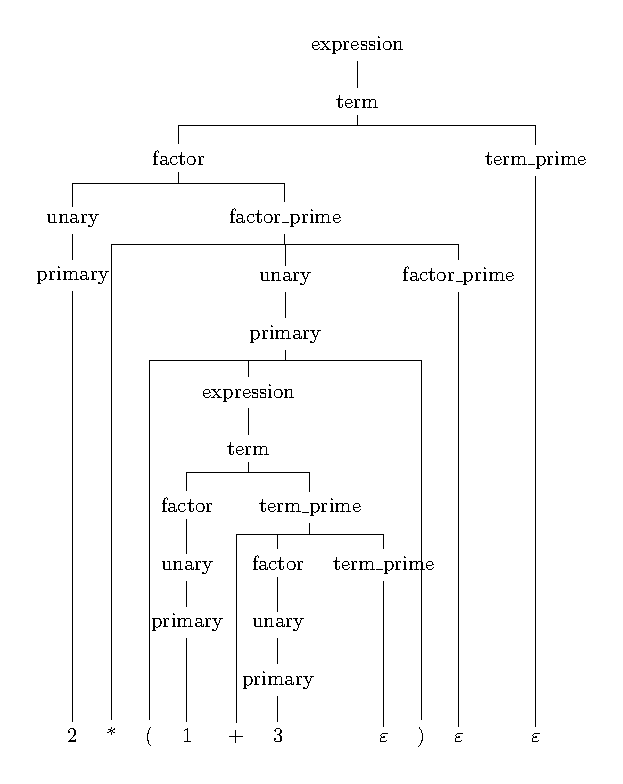
\includegraphics[width=0.75\textwidth]{figures/parse-example.pdf}
  \caption{Example parse tree for the expression $2*(1+3)$.}
\end{figure}

The example above shows the parsing process and how a lower-precedence operator is not attempted to be parsed until all higher-precedence levels have been fully reduced (via their \texttt{\_prime} and $\varepsilon$-branches), the grammar structure ensures, for example, that $*$ binds tighter than $+$, and that $+$ binds tighter than $==$. Parentheses are handled in \texttt{primary}, letting the parser suspend this fixed precedence ordering and recursively parse a new full expression inside. To sum up, the $\varepsilon$-productions terminate each level's repetition, while the layering of nonterminals enforces both the precedence tiers and the correct associativity for every operator.


The grammar is implemented as a standalone class. The \texttt{Grammar} class is written in an abstract manner, allowing it to hold information about the Lumerical Scripting Language, while staying extendable. To facilitate this, the \texttt{Grammar} class holds a list of productions. The productions are represented as a separate \texttt{Production} classes holding information about the \gls{lhs} and \gls{rhs} of the production. The \gls{lhs} is a single nonterminal, while the \gls{rhs} is a list of nonterminals, terminals, actions, or a $\varepsilon$ symbol. The \texttt{Production} class also keeps track of the production number, assigning each production a unique numerical value in an ascending fashion and whether the production is nullable.

Circling back to the \texttt{Grammar} class, it also provides helper functions, such as \texttt{append}, which adds the passed production to the grammar, while also updating the \texttt{nullable} attribute of the production. The \texttt{Grammar} class also provides \texttt{terminals} and \texttt{nonterminals} methods, to list all terminals and nonterminals in the grammar.


\section{Lexical Analysis}
After defining a grammar, the first stage in creating a transpiler is the lexer. There are multiple methods in which a lexer may be modeled, the most straight-forward being the use of a \gls{dfa} formalism and a loop over all input characters while checking if there is a valid production from the current character to the look-ahead character and greedily continue and backtrack to the last successful match upon not being able to find an applicable production.

\begingroup
\vspace{1.5em}
\begin{algorithm}[H]
\setlength{\algomargin}{1.5em}
current\_state $\gets$ \texttt{None}\\
last\_accepting\_state $\gets$ \texttt{None}

    \While{look-ahead\_character != EOF}{
        \If{has\_transition(current\_state, look-ahead)}{
            current\_state $\gets$ \text{next\_state}(current\_state, look-ahead)\\
            get\_next\_character()
            
            \If{\text{is\_accepting\_state}(current\_state)}{
                last\_accepting\_state $\gets$ current\_state
            }
        }
        \Else{
            \If{no\_accepting\_state\_visited}{

				\Return{\texttt{None}} \tcp*{Failure} 
            }
            \Else{
				revert\_to\_previous\_accepting\_state\_and\_revert\_input\_characters
				\Return{current\_state} \tcp*{Success} 
            }
        }
    }
    


\caption{State Machine Based Lexer.}
\label{alg:lexer-state-based}
\end{algorithm}
\vspace{1.5em}
\endgroup

This implementation is fine, how-ever, with an ever-growing number of states, which have to be hard-coded; the solution may become rather complex. Indeed, a cleaner method exists. Since any \gls{dfa} may be transformed into a regular expression, it is sufficient to try to match all regular expressions against the input and return the longest match while removing it from the input. 


\begingroup
\vspace{1.5em}
\begin{algorithm}[H]
\setlength{\algomargin}{1.5em}
longest\_match $\gets$ \texttt{None}\\


    \For{all\_regular\_expressions}{
        \If{regular\_expression\_matches\_input}{
            \If{regular\_expression\_is\_longer\_than\_longest\_match}{
                longest\_match $\gets$ current\_regular\_expression
            }
        }
    }
    \If{longest\_match != \texttt{None}}{
		\Return{matching\_token}    
		remove\_matched\_lexeme\_from\_input
    }
    \Else{
    		\Return{\texttt{None}} \tcp*{Failure} 
    }
    


\caption{Regular Expression Based Lexer.}
\label{alg:lexer-expression-based}
\end{algorithm}
\vspace{1.5em}
\endgroup

This approach is not only more straight forward, but also allows modeling the lexer in a more pythonic manor. Each token is represented as a unique class with holds the regular expression pattern matching the corresponding token. Each specific token class inherits a common token class, after that, it is sufficient for the lexer to enumerate over all children of the token class and search for the one with the longest match resulting in a greedily matched token.


This is reflected in the \texttt{Lexer} class, which provides a stream of tokens. The class holds information about the source code, which is to be processed. This is achieved through \texttt{source} attribute and a \texttt{cursor} attribute, which is incremented as the source code is parsed. The \texttt{Lexer} class implements a \texttt{tokens} generator, which repetitively calls \texttt{advance} and yields the tokens, until all are exhausted, while discarding white space tokens, such as a new line and space tokens. 

The \texttt{advance} method returns a single token, or the None value, when the end of the input is reached. Otherwise it greedily matches the longes token as described in Algorithm~\ref{alg:lexer-expression-based}. This is achieved by iterating over all tokens, which are obtained by retrieving all subclasses og the \texttt{Token} class, as each individual token is a child class.

The \texttt{Token} class holds information about a token, such as the name, given by the class \texttt{\_\_name\_\_} method. The lexeme pattern, used to match the token, is stored as a regular expression. The \texttt{token} class also stores the lexeme, which it matched. This is used during logging and also mainly for storing the value of literals, such a strings, integers and floats which are used during the code generation phase.


\section{LL Parser}
A \gls{ll} grammar was chosen due to the reasons described in \cref{grammar}, specifically a \gls{ll} (1) grammar. There are two common implementations of parsers that accept \gls{ll} (1) grammars. The first being a recursive descent parser. It is a kind of top-down parser, that models the parsed grammar in such a fashion, that each nonterminal of the grammar is represented by a procedure in code. The methods recurse and invoke each other, parsing the grammar. This is a simple procedure to implement, however often resulting in long code that is proportional to the size of the grammar, which makes it harder to comprehend and easier introduce mistakes in the implementation. This does not pair well with the future possible extensions of this transpiler to cover the entirety Lumerical's scripting language.

The second method is a \gls{ll} table based parser. It is a deterministic pushdown automaton utilizing a stack and a parsing table. It continually expands the leftmost nonterminal in a derivation with a look-ahead of one token to chose the correct production from the parsing table. It starts by reading a token from the lexer and looking at the top most item on the stack, in the case of a nonterminal, the corresponding production from the parsing table, given by the nonterminal and terminal, is pushed on the stack. If no production is found, a parsing error is raised. On the other hand, if the top stack symbol is a terminal, it must match the input terminal, otherwise a parsing error is raised. This notion is shown in alg.~\ref{alg:parser} based on~\cite[Table 4.12.]{Holub_1990}.
based parser. It is a deterministic pushdown automaton utilizing a stack and a parsing table. It continually expands the leftmost nonterminal in a derivation with a look-ahead of one token to chose the correct production from the parsing table. It starts by reading a token from the lexer and looking at the top most item on the stack, in the case of a nonterminal, the corresponding production from the parsing table, given by the nonterminal and terminal, is pushed on the stack. If no production is found, a parsing error is raised. On the other hand, if the top stack symbol is a terminal, it must match the input terminal, otherwise a parsing error is raised. This 
\begingroup
\vspace{1.5em}
\begin{algorithm}[H]\label{alg:parser}
  \setlength{\algomargin}{1.5em}

  initialize stack with root grammar nonterminal
  \While{parse stack not empty}{
    \If{top symbol is nonterminal}{
      what\_to\_push = parse\_table[top symbol][current input token]\\
      \If{what\_to\_push == None}{
        \text{Syntax error.}
      }
      \Else{
        add reversed what\_to\_push to stack
      }
    }
    \ElseIf{top symbol is terminal}{
      \If{top symbol == current input token}{
        \If{current input token != end of file}{
          get next token
        }
      }
      \Else{
        \text{Syntax error.}
      }
    }
  }

\caption{Top-down table based parsing algorithm.}
\end{algorithm}
\vspace{1.5em}
\endgroup

The theory of a parsing table is pretty straight forward. Each production in the grammar 
In a parsing table, each row corresponds to a nonterminal and each column to a terminal. The cell at the intersection of a row and column contains the production to be applied. If no production is found, a parsing error is raised. A simple example of a \gls{ll}(1) grammar is provided in Figure~\ref{tab:example-bfn-ll} and the corresponding parsing table in Table~\ref{tab:example-ll-table}.

%\begin{table}[H]
%\centering
%\begin{tabular}{l|rcl}
%1. & stmt   & $\rightarrow$ & expr \textbf{SEMI}        \\
%2. & expr   & $\rightarrow$ & factor \textbf{PLUS} expr \\
%3. &        & |             & factor                    \\
%4. & factor & $\rightarrow$ & \textbf{NUMBER}          
%\end{tabular}
%\caption{Simple example \gls{bnf} grammar that is not \gls{ll}(1).}
%\label{tab:example-bfn}
%\end{table}
\begin{figure}[H]
\centering
\begin{table}[H]
\centering
\begin{tabular}{l|rcl}
1. & stmt       & $\rightarrow$ & expr \textbf{SEMI}			\\
2. & expr       & $\rightarrow$ & factor expr\_tail			\\
3. & expr\_tail & $\rightarrow$ & \textbf{PLUS} expr			\\
4. &            & |             & $\varepsilon$					\\
5. & factor     & $\rightarrow$ & \textbf{NUMBER}          
\end{tabular}
\label{tab:example-bfn-ll}
\end{table}
\caption{Simple example \gls{bnf} grammar that is \gls{ll}(1).}
\end{figure}

\begin{table}[H]
  \centering
  \begin{tabular}{|l|c|c|c|}
\hline
              &\textbf{SEMI}  &\textbf{PLUS}  &\textbf{NUMBER}  \\
\hline
  stmt        &               &               &1                \\
\hline
  expr        &               &               &2                \\
\hline
  expr\_tail  &4              &3              &                 \\
\hline
  factor      &               &               &5                \\
\hline
  \end{tabular}
  \caption{Example \gls{ll}(1) parsing table based on the grammar in Figure~\ref{tab:example-bfn-ll}.}
  \label{tab:example-ll-table}
\end{table}

\subsection{LL Table Construction}
\gls{ll} (1) parse tables are constructed using the FIRST, FOLLOW and SELECT sets, which are solved for each nonterminal. The FIRST set of a nonterminal consists of all terminal symbols that can appear at the beginning of any string derivable from that nonterminal.

The FIRST sets are evaluated in an iterative process for the whole grammar. The set is evaluated for each nonterminal present in the grammar, always updating the corresponding set by preforming a FIRST closure, until each nonterminal's FIRST set does not change. The theoretical approach it detailed below. In the following sections, $\varepsilon$ will be treated as a terminal symbol as a simplification, even though it is not, and LHS and RHS will correspond to. 


\begingroup
\vspace{1.5em}
\begin{algorithm}[H]
  \setlength{\algomargin}{1.5em}
  \If{production is nullable}{
    \Return{}
  }
  \For{symbol in production.RHS}{
    \If{symbol is terminal}{
      add symbol to first[production.LHS]\\
      \Return{}
    }
    \Else{
      add first[symbol] to first[production.LHS]\\
      \If{symbol is not nullable}{
        \Return{}
      }
    }
  }


\caption{The FIRST closure algorithm.}
\label{alg:first-closure}
\end{algorithm}
\vspace{1.5em}
\endgroup

Algorithm~\ref{alg:first-closure} corresponds to a generalized rule for calculating the FIRST set. For a production in the form of $s \rightarrow \alpha \mathcal{B} \beta$, where $s$ is the nonterminal, for which the FIRST set is being calculated, $\alpha$ are 0 or more nullable\footnote{As a reminder, a nonterminal is \emph{nullable} if it can be transformed to $\varepsilon$ by some production, i.e.\ there has to be at least one production of the form $s \rightarrow \varepsilon$, where $s$ is a nonterminal.} nonterminals, $\mathcal{B}$ is a single terminal or nonterminal and $\beta$ are multiple terminals or nonterminals. Then the FIRST$(s)$ set is the union of FIRST$(\beta)$ and FIRST$(\alpha)$ sets~\cite[Chapter~4.7.1]{Holub_1990}.


Similarly to the FIRST sets, the FOLLOW are computed incrementally, until nop change in the sets is observed. The FOLLOW contains those terminals, which may follow the nonterminal, for which the FOLLOW set is evaluated. 

\begingroup
\vspace{1.5em}
\begin{algorithm}[H]
  \setlength{\algomargin}{1.5em}
  \If{production is nullable}{
    \Return{}
  }
  \For{\text{symbol} in \text{production.RHS}}{
    \If{symbol is terminal}{
        \textbf{continue}
    }
    \Else{
      \If{next\_symbol is terminal}{
        add next\_symbol to follow[symbol]\\
      }
      \Else{
        add first[next\_symbol] to follow[symbol]\\
      }
    }
  }
  \For{symbol in reversed production.RHS}{
    \If{symbol is terminal}{
      \textbf{break}
    }
    \Else{
      last\_nonterminal = symbol\\
      add follow[production.LHS] to follow[symbol]\\
      \If{symbol is not nullable}{
        \textbf{break}
      }
    }
  }
  \If{\text{last\_nonterminal}}{
    add follow[production.LHS] to follow[last\_nonterminal]
  }

  \caption{The FOLLOW closure algorithm.}
  \label{alg:follow-closure}
\end{algorithm}
\vspace{1.5em}
\endgroup
Algorithm~\ref{alg:follow-closure} provides a general method for computing the FOLLOW set. Consider a production expressed as $s \rightarrow \dots a \alpha \mathcal{B}\dots$, where $s$ and $a$ are nonterminals, $\alpha$ is a possibly empty sequence of nullable nonterminals, and $\mathcal{B}$ is a terminal or nonterminal. FOLLOW($a$) is updated with the union of FIRST($\alpha$) and FIRST($\mathcal{B}$)~\cite[Chapter~4.7.2]{Holub_1990}.

Finally we need to calculate the SELECT sets (also know as PREDICT), unlike with the previous two cases, the SELECT sets ale calculated in one pass. The \gls{ll}(1) SELECT set for a production rule consists of all input symbols that can appear as the next token in the input stream when that production is correctly applied.



\begingroup
\vspace{1.5em}
\begin{algorithm}[H]
  \setlength{\algomargin}{1.5em}
  \For{production in productions}{
    \For{symbol in production.RHS}{
      \If{symbol is nonterminal}{
        add first[symbol] to select[production]
      }
      add follow[production.LHS] to select[production]\\
      \If{symbol is nonterminal}{
        add follow[production.LHS] to first[production]\\
        \If{symbol is not nullable}{
          \textbf{break}
        }
      }
      \Else{
        add symbol to select[production]\\
        \textbf{break}
      }
    }
  }
  
  \caption{The \gls{ll}(1) SELECT algorithm.}
  \label{alg:select-closure}
\end{algorithm}
\vspace{1.5em}
\endgroup

Algorithm~\ref{alg:select-closure} outlines a general procedure for computing the \gls{ll}(1) SELECT set which corresponds to the following formal definition. When dealing with a \underline{non-nullable}\footnote{The opposite of a nullable production—that is, a production whose right-hand side is not solely $\varepsilon$, nor composed entirely of symbols that can derive $\varepsilon$ through some sequence of derivations.
} production of the form $s\rightarrow \alpha \mathcal{B} \dots$, where $s$ is a nonterminal, $\alpha$ is a sequence of one or more nullable nonterminals, and $\mathcal{B}$ is either a terminal or a non-nullable nonterminal (i.e., one that cannot derive $\varepsilon$), possibly followed by additional symbols. The \gls{ll}(1) SELECT set for this production is the union of FIRST($\alpha$) and FIRST($\mathcal{B}$).
On the other hand, when a nullable production is encountered in the following form $s\rightarrow \alpha$, where $s$ is a nonterminal, $\alpha$ denotes a sequence comprising zero or more occurrences of nullable nonterminals. The union of FIRST($\alpha$) and FOLLOW($s$) is added to the \gls{ll}(1) SELECT set for the production~\cite[Chapter~4.7.3]{Holub_1990}.


After obtaining the \gls{ll}(1) SELECT sets for the grammar, the construction of the \gls{ll} parsing table is trivial. 

\begingroup
\vspace{1.5em}
\begin{algorithm}[H]\label{alg:select-to-table}
  \setlength{\algomargin}{1.5em}
  initialize table to error states
  \For{production in productions}{
    \For{token in select[production]}{
      table[production.LHS][token] = production
    }
  }
  
  \caption{Translation of \gls{ll}(1) SELECT sets to a parse table.}
\end{algorithm}
\vspace{1.5em}
\endgroup


This approach is implemented in the \texttt{LLTable} class. The class is instanced using the grammar for which it calculates the first, follow, and predict sets. This is handled in \texttt{ComputeFirstSets}, which calls \texttt{FirstClosure} until the are no more changes, as described above. Following that, \texttt{ComputeFollowSets} is called, which as in the case of first sets, calls is respective function \texttt{FollowClosure} until no more changes are made to the follow sets. As the last preliminary step, the select sets are computed using the \texttt{ComputeSelectSets} function. 



\section{Code Generation}\label{sec:code-generation}

Up to this point, we have applied multiple steps of the transpilation process, such as splitting the input code into tokens, creating a \gls{ll}(1) parsing table and using it to parse the input code. Thus so far, we have verified that the input code is a valid Lumerical Scripting Language\footnote{As discussed a in \cref{sem-analysis} on p.~\pageref{sem-analysis}, the input code is expected to be semantically correct. This can be simply verified by executing the code in Lumerical.}, however we have not created any resulting Python code. This is where the concept of \emph{actions} is introduced~\cite{Holub_1990}.

Actions are symbols added to the grammar, they act as a terminal symbol, in the sense that they do not get expanded, however they do not consume a token from the input upon being matched. On the contrary, actions store logic that is executed at specific points in the grammar, which is used for generating the resulting Python code.

Actions are implemented as a separate \texttt{Action} class, which have a abstract method \texttt{call}, when the parser processes a action, it automatically invokes this aforementioned \texttt{call} method.

\subsection{Python AST}

As mentioned above in \cref{grammar}, Python contains a built in module called \texttt{ast}\footnote{\url{https://docs.python.org/3/library/ast.html}}. This module help with processing Python code, generating \glspl{ast} out of Python code and most importantly also generating Python code from a \gls{ast}. For clarity all \gls{ast} node provided by the Python \texttt{ast} module will be prepended with \texttt{ast.}.

Python \texttt{ast} module provides a root node named \texttt{ast.Module} that has an attribute \texttt{body}, which is a list of the module statements. This is the node we will build upon in the parsing process by adding statements we parse to the \texttt{ast.Module}. 
Thus extending the alg.~\ref{alg:parser} with the option to accept actions in the grammar, whose full form containing actions is listed in Appendix~\ref{appendix:two}, we get the final version of the top-down table based parser as seen in alg.~\ref{alg:parser-actions} bellow.



\begingroup
\vspace{1.5em}
\begin{algorithm}[H]\label{alg:parser-actions}
  \setlength{\algomargin}{1.5em}
  initialize stack with root grammar nonterminal\\
  \textcolor{red}{initialize value\_stack with Module node}\\
  \textcolor{red}{initialize empty token\_stack }

  \While{parse stack not empty}{
    \If{top symbol is nonterminal}{
      what\_to\_push = parse\_table[top symbol][current input token]\\
      \If{what\_to\_push == None}{
        \text{Syntax error.}
      }
      \Else{
        add reversed what\_to\_push to stack
      }
    }
    \ElseIf{top symbol is terminal}{
      \If{top symbol == current input token}{
        \If{current input token != end of file}{
          \textcolor{red}{put token on token\_stack}\\
          get next token
        }
      }
      \Else{
        \text{Syntax error.}
      }
    }
    \textcolor{red}{
    \Else{
      invoke action call function with value\_stack and  token\_stack
      }
    }
  }

\caption{Top-down table based parsing algorithm extended with actions.}
\end{algorithm}
\vspace{1.5em}

The changes to the previous algorithm are highlighted in red, namely the addition of \texttt{value\_stack}, \texttt{token\_stack}, and the action conditional branch. The \texttt{value\_stack} is used to store the \gls{ast} node, however a simple variable is not sufficient because of cases, when the whole expression is not ney parsed, thus a last-in first-out queue is used. This allows node which are not yet fully parsed to be pushed on the stack and popped once they may be complete. The \texttt{token\_stack} is used mainly as a way, for the actions to also access the token which were parsed. This is not necessary for tokens such as keywords and other syntactic sugar\footnote{\url{https://en.wikipedia.org/wiki/Syntactic_sugar}\todo{is OK?}}, however when facing tokens with semantic meaning such as integers, strings and other, their lexeme carries important information which is used during generation. Both of these are expected by all action \texttt{call} methods even though the \texttt{token\_stack} is used sparsely a uniform interface was deemed desirable.

\subsection{Actions}
An exhaustive description of every implemented action would be excessively laborious and contribute little of meaningful value. However a overview of the implementation techniques and key examples will be provided in this sub section.

\paragraph{Anathomy of an Action}
Actions were generally separated in to 3 parts:
\begin{itemize}
  \item \textbf{Extraction Phase:} The stack values are read and popped into local variables.
  \item \textbf{Construction Phase:} The AST node is created using the extracted values.
  \item \textbf{Restoration Phase:} The newly constructed node is returned and the stack is reordered.
\end{itemize}

\paragraph{StoreToBody}
The most commonly used action is \texttt{StoreToBody}. As mentioned before, the \texttt{ast.Module} that has an attribute \texttt{body}, however this is not the only, many other such as the \texttt{ast.If}, \texttt{ast.Else}, \texttt{ast.For} and other each have a \texttt{body} attribute. This action expects the \texttt{value\_stack} to contain a node on the top, this will be the node we store to the \texttt{body} of the second node bellow it on the stack. Both of the node are popped of, the top node is appended to the \texttt{body} list of the node bellow and that node is pushed back on the stack. This allows us to prepare nodes in advance and then add them to the body of the scope once the whole node was parsed.

\begin{figure}[H]\label{fig:storetobody-stack}
  \centering
  {\small

  \begin{tabular}{|c|}
    \hline
    \textbf{Stack Before} \\ \hline
    \texttt{\tiny{ast.}}\texttt{Break}\\ \hline
    \texttt{\tiny{ast.}}\texttt{For(body=[\dots])} \\ \hline
    \(\dots\)             \\ \hline
  \end{tabular}
  \hspace{0.25em}$\Longrightarrow$\hspace{0.25em}
  \begin{tabular}{|c|}
    \hline
    \textbf{Stack After} \\ \hline
    \texttt{\tiny{ast.}}\texttt{For(body=[\dots,}\texttt{\tiny{ast.}}\texttt{Break])} \\ \hline
    \(\dots\)                       \\ \hline
  \end{tabular}
  }
  \caption{LIFO value stack before and after applying \texttt{StoreToBody}.}
  
\end{figure}

\paragraph{StoreLiteral}
The \texttt{StoreLiteral} is on of the few actions, that also utilize the initialization method, simply accepting a type value derived from the grammar later used for the conversion which will be described soon. When called, the action first pops a value of the \texttt{token\_stack}, this is the literal pushed onto the \texttt{token\_stack} by the parser. Then an attempt is made to convert the string representation to a built-in Python type as specified in the initialization function. Following this a \texttt{ast.Constant} node is created. This will store the converted value as its \texttt{value} attribute and it is pushed on the stack. \texttt{StoreLiteral} is called after parsing a literal in the  grammar.

\begin{figure}[H]\label{fig:storeliteral-stack}
  \centering
  {\small

  % Token stack
  \begin{tabular}{|c|}
    \hline
    \textbf{Token Stack} \\ \hline
    \texttt{"123"}       \\ \hline
    \(\dots\)            \\ \hline
  \end{tabular}
  \begin{tabular}{|c}
    \\
    \\
    \\
    \\
  \end{tabular}
  % Stack Before
  \begin{tabular}{|c|}
    \hline
    \textbf{Stack Before} \\ \hline
    \(\dots\)             \\ \hline
  \end{tabular}
  \hspace{0.25em}$\Longrightarrow$\hspace{0.25em}
  % Stack After
  \begin{tabular}{|c|}
    \hline
    \textbf{Stack After} \\ \hline
    \texttt{\tiny{ast.}}\texttt{Constant(value=123)} \\ \hline
    \(\dots\)                       \\ \hline
  \end{tabular}
  }
  \caption{LIFO value stack before and after applying \texttt{StoreLiteral}.}
  
\end{figure}

\paragraph{StoreVariableName}
\texttt{StoreVariableName} is a helper action. It pops a variable name from the token stack and converts it to a \texttt{ast.Name} which is used e.g. for assigning values to variables. The \texttt{ast.Name} context is set to store.

\begin{figure}[H]\label{fig:storeVariableName-stack}
  \centering
  {\small

  % Token stack
  \begin{tabular}{|c|}
    \hline
    \textbf{Token Stack} \\ \hline
    \texttt{"x"}       \\ \hline
    \(\dots\)            \\ \hline
  \end{tabular}
  \begin{tabular}{|c}
    \\
    \\
    \\
    \\
  \end{tabular}
  % Stack Before
  \begin{tabular}{|c|}
    \hline
    \textbf{Stack Before} \\ \hline
    \(\dots\)             \\ \hline
  \end{tabular}
  \hspace{0.25em}$\Longrightarrow$\hspace{0.25em}
  % Stack After
  \begin{tabular}{|c|}
    \hline
    \textbf{Stack After} \\ \hline
    \texttt{\tiny{ast.}}\texttt{Name(id="x",ctx=}\texttt{\tiny{ast.}}\texttt{Store())} \\ \hline
    \(\dots\)                       \\ \hline
  \end{tabular}
  }
  \caption{LIFO value stack before and after applying \texttt{StoreVariableName}.}
  
\end{figure}

\paragraph{AssignToVariable}
The \texttt{AssignToVariable} is used to assign a value to a variable. It is called after the whole expression was parsed. The action expects a value, typically \texttt{ast.Const}, on top of the stack. Next, a second node is popped from the stack, and it must be an \texttt{ast.Name}. Once both the name and value are acquired a \texttt{ast.Assign} node is created and pushed on the stack.

\begin{figure}[H]\label{fig:assignToVariable-stack}
  \centering
  {\small

  \begin{tabular}{|c|}
    \hline
    \textbf{Stack Before} \\ \hline
    \texttt{\tiny{ast.}}\texttt{Constant(value="text")}\\ \hline
    \texttt{\tiny{ast.}}\texttt{Name(id="var",}\\
    \texttt{ctx=}\texttt{\tiny{ast.}}\texttt{Store())} \\ \hline
    \(\dots\)             \\ \hline
  \end{tabular}
  \hspace{0.25em}$\Longrightarrow$\hspace{0.25em}
  \begin{tabular}{|c|}
    \hline
    \textbf{Stack After} \\ \hline
    \texttt{\tiny{ast.}}\texttt{Assign(targets=[}\texttt{\tiny{ast.}}\texttt{Name],}\\
    \texttt{value=}\texttt{\tiny{ast.}}\texttt{Const)} \\ \hline
    \(\dots\)                       \\ \hline
  \end{tabular}
  }
  \caption{LIFO value stack before and after applying \texttt{AssignToVariable}.}
  
\end{figure}

\paragraph{BinaryOperation}
Previously, we examined the creation of constants and their assignment to variables, and we also presented an example parse of an expression in Figure~\ref{fig:parse-example} (page~\pageref{fig:parse-example}). A binary operation, as is implied from its name, expect two operands --- expressions. The right operand was parsed later, thus it will appear on top. Following that the left operand is also popped of the stack. To decide which operator to use, a \texttt{ast.operator} is passed into initialization function of the action. After obtaining both operands and the operator a \texttt{ast.BinOp} node is constructed and pushen on the stack.

\begin{figure}[H]\label{fig:binaryOperation-stack}
  \centering
  {\small

  \begin{tabular}{|c|}
    \hline
    \textbf{Stack Before} \\ \hline
    \texttt{\tiny{ast.}}\texttt{Constant(value=1)}\\ \hline
    \texttt{\tiny{ast.}}\texttt{Constant(value=2)}\\ \hline
    \(\dots\)             \\ \hline
  \end{tabular}
  \hspace{0.25em}$\Longrightarrow$\hspace{0.25em}
  \begin{tabular}{|c|}
    \hline
    \textbf{Stack After} \\ \hline
    \texttt{\tiny{ast.}}\texttt{BinOp(}\texttt{\tiny{ast.}}\texttt{Constant(value=2),}\\
    \texttt{\tiny{ast.}}\texttt{Add(),}\texttt{\tiny{ast.}}\texttt{Constant(value=1))} \\ \hline
    \(\dots\)                       \\ \hline
  \end{tabular}
  }
  \caption{LIFO value stack before and after applying \texttt{BinaryOperation}.}
  \label{fig:binaryOperation-stack}
\end{figure}

Boolean logic operators are implemented similarly, however their operands are added as a list due to Python's design, e.g. \texttt{ast.BoolOp(op=self.op, values=[left, right])}. Unary operators are implemented by popping the value of the stack, and pushing it as e.g. \texttt{ast.UnaryOp(op=USub(), operand=operand)}.

\paragraph{If}
The \texttt{If} action constructs the first part of a conditional statement, the \texttt{if} branch. However to properly explain how later \texttt{elif} and \texttt{else} branches are constructed, an overview of how Python \texttt{ast} parses conditional statements\footnote{\url{https://docs.python.org/3/library/ast.html\#control-flow}} is necessary. This is best shown on the example bellow.

\begin{figure}[htbp]\label{fig:python-if-ast}
  \centering

  \begin{subfigure}[t]{0.48\textwidth}
    \begin{lstlisting}[style=python]
If(
  test=a,
  body=[Constant(value=1)],
  orelse=[
    If(
      test=b,
      body=[Constant(value=2)],
      orelse=[Constant(value=3)]
    )
  ]
)
    \end{lstlisting}
    \caption{AST representation}
  \end{subfigure}
  \hfill
  \begin{subfigure}[t]{0.4\textwidth}
    \begin{lstlisting}[style=python]
if a:
    1
elif b:
    2
else:
    3
    \end{lstlisting}
    \caption{Python source code}
  \end{subfigure}

  \caption{A conditional Python statement and its corresponding AST structure.}
  
\end{figure}

The initial \texttt{if} branch contains a \texttt{test} attribute which has to evaluate to \texttt{True} for the first \texttt{body} to be executed. If the \texttt{orelse} attribute is empty, the previous statement was a single \texttt{if}, however is the attribute contains nodes other than another \texttt{ast.If} node, they are executed as part of the \texttt{else} path of the conditional statement. On the contrary, if the \texttt{orelse} attribute of the initial \texttt{ast.If} node contains a nested \texttt{ast.If}, it is treated as a \texttt{elif}. This can be repeated indefinitely.

With an understanding of Python \texttt{ast} control flow, we now return to the implementation of the \texttt{If} action, which pops a value of the stack. This is the expression that will be evaluated as the test. Following this a \texttt{ast.If} node is created, the expression is passed to the \texttt{test} attribute and the node is pushed on the stack.

\begin{figure}[H]\label{fig:if-stack}
  \centering
  {\small

  \begin{tabular}{|c|}
    \hline
    \textbf{Stack Before} \\ \hline
    \texttt{\tiny{ast.}}\texttt{Expression()}\\ \hline
    \(\dots\)             \\ \hline
  \end{tabular}
  \hspace{0.25em}$\Longrightarrow$\hspace{0.25em}
  \begin{tabular}{|c|}
    \hline
    \textbf{Stack After} \\ \hline
    \texttt{\tiny{ast.}}\texttt{If(body=[],orelse=[],}\\
    \texttt{test=}\texttt{\tiny{ast.}}\texttt{Expression())} \\ \hline
    \(\dots\)                       \\ \hline
  \end{tabular}
  }
  \caption{LIFO value stack before and after applying \texttt{If} action.}
  
\end{figure}

\paragraph{StoreToElse}
An attentive reader may have noticed, that we need to add nodes not only to the \texttt{body} of the \texttt{ast.If} but also to the \texttt{orelse}. However our \texttt{StoreToBody} only stores to the \texttt{body}, this is where \texttt{StoreToElse} is utilized. That said, there are two cases that have to be handled, the first of which is when we are storing a node to the terminal \texttt{else}.

To begin with we pop the target node from the stack, this will become part of the \texttt{orelse}, following that we pop a second value of the stack, it is a \texttt{ast.If} node. If it were an expression, the second case would occur. Once the \texttt{ast.If} node and the target node have been obtained, we recursively traverse the \texttt{ast.If} node's \texttt{orelse} attribute. If \texttt{orelse} contains another \texttt{ast.If}, the traversal continues until we encounter an \texttt{ast.If} whose \texttt{orelse} is not itself an \texttt{ast.If}. At that deepest level, we append the target node to its \texttt{orelse} list and push the \texttt{ast.If} node on the stack.
\begin{figure}[H]\label{fig:storeToElse-stack-1}
  \centering
  {\small
  \begin{tabular}{|c|}
    \hline
    \textbf{Stack Before} \\ \hline
    \texttt{\tiny{ast.}}\texttt{Constant()}\\ \hline
    \texttt{\tiny{ast.}}\texttt{If(body=[\dots], orelse=[\dots])}\\ \hline
    \(\dots\)             \\ \hline
  \end{tabular}
  \hspace{0.25em}$\Longrightarrow$\hspace{0.25em}
  \begin{tabular}{|c|}
    \hline
    \textbf{Stack After} \\ \hline
    \texttt{\tiny{ast.}}\texttt{If(body=[\dots],}\\
    \texttt{orelse=[\dots, }\texttt{\tiny{ast.}}\texttt{Constant()])}\\ \hline
    \(\dots\)                       \\ \hline
  \end{tabular}
  }
  \caption{LIFO value stack before and after applying \texttt{StoreToElse} action in the first case.}
  
\end{figure}

In the second case, following the first popped target node a \texttt{ast.Expression} is encountered, this is the test for the \texttt{elif}, thus we pop a final node, now the \texttt{ast.If}. Similarly as before, we recurse to the deepest \texttt{ast.If} and we append the target node to its \texttt{body} list. This node is pushed on the stack, but the \texttt{ast.Expression} cannot be consumed by this action, as then we could not add multiple statement, thus the \texttt{ast.Expression} is preserver and pushed on the stack.

\begin{figure}[H]\label{fig:storeToElse-stack-2}
  \centering
  {\small
  \begin{tabular}{|c|}
    \hline
    \textbf{Stack Before} \\ \hline
    \texttt{\tiny{ast.}}\texttt{Constant()}\\ \hline
    \texttt{\tiny{ast.}}\texttt{Expression()}\\ \hline
    \texttt{\tiny{ast.}}\texttt{If(body=[\dots], orelse=[\dots])}\\ \hline
    \(\dots\)             \\ \hline
  \end{tabular}
  \hspace{0.25em}$\Longrightarrow$\hspace{0.25em}
  \begin{tabular}{|c|}
    \hline
    \textbf{Stack After} \\ \hline
    \texttt{\tiny{ast.}}\texttt{Expression()}\\ \hline
    \texttt{\tiny{ast.}}\texttt{If(body=[\dots, }\\
    \texttt{\tiny{ast.}}\texttt{Constant()], orelse=[\dots])}\\ \hline
    \(\dots\)                       \\ \hline
  \end{tabular}
  }
  \caption{LIFO value stack before and after applying \texttt{StoreToElse} action in the second case.}
  
\end{figure}

\texttt{HandleElse} and \texttt{HandleElseCleanup} do not constitute their own section, however a quick overview of the \texttt{HandleElse} is as follows. The action pop an item of the stack, in case it is a \texttt{ast.If}, it is returned and nothing is done. In case it is an \texttt{ast.Expression}, a second node which is now a \texttt{ast.If} is popped, the expression is set as the node's \texttt{test} attribute and both are returned, such that the expression is on top.
At the end of the whole \texttt{if}-\texttt{elif}\texttt{else} chain, \texttt{HandleElseCleanup} is invoked searching for an \texttt{ast.Expression} as the top node and discarding it.


\paragraph{Loops}
Other forms of control structures are \texttt{for} and \texttt{while} loops. Lumerical does not support while loops as discussed during the construction of the grammar however they substitute them with \texttt{for} loops in the form of \texttt{for(0; conditional\_expression; 0) \{\}} as per the documentation~\cite{ansys_for_command}. However, since Lumerical permits arbitrary modification of the loop's stop-condition variable within the loop body, using Python \texttt{for} loops to implement Lumerical \texttt{for} loops is not feasible even though Lumerical provides a range notation. Thus all loops are implemented as \texttt{while} loops in Python. The following actions help creating the \texttt{while} loop and properly accepting both range and "C" style forms of loops e.g.:
\begin{itemize}
  \item  \texttt{for(x=1:2:100) \{\}}
  \item  \texttt{for(x=1; x<= 100; x=x+2) \{\}}
\end{itemize}

\paragraph{CreateEmptyWhile}
The \texttt{CreateEmptyWhile} simply creates an empty \texttt{ast.While} and pushes it on the stack as later actions expect a \texttt{ast.While} node present. Both loop styles are accepted in the \texttt{loop\_condition} nonterminal in production 42 and 43 on page~\pageref{tab:commands4}. The first type of loops we will tackle is the range style. This is handled by the \texttt{CreateRangeCondition}; there are two cases to consider, when the range is only composed of two values (\emph{start:stop}) or when an step is added (\emph{start:step:stop}). The \texttt{end} value is popped of the stack, an \texttt{ast.Assign} node is always present with the first part of the range, i.e. the \texttt{start} value which is also popped. A \texttt{ast.Compare} node is created to serve as the terminating condition for the \texttt{ast.While} node. This involves comparing the value of the \texttt{ast.Assign} variable to the \texttt{end} value. An \texttt{ast.AugAssign} is also created, this serves as the incrementation that will happen during each loop iteration and by default with a step of $1$. The \texttt{test} attribute of \texttt{ast.While} is updated, then the \texttt{ast.Assign} is pushed, followed by \texttt{ast.AugAssign} and \texttt{ast.While}.

\begin{figure}[H]\label{fig:createEmptyWhile-stack}
  \centering
  {\small
  \begin{tabular}{|c|}
    \hline
    \textbf{Stack Before} \\ \hline
    \texttt{\tiny{ast.}}\texttt{Constant(value=10)}\\ \hline
    \texttt{\tiny{ast.}}\texttt{Assign(target="x", value=1)}\\ \hline
    \texttt{\tiny{ast.}}\texttt{While()}\\ \hline
    \(\dots\)             \\ \hline
  \end{tabular}
  \hspace{0.25em}$\Longrightarrow$\hspace{0.25em}
  \begin{tabular}{|c|}
    \hline
    \textbf{Stack After} \\ \hline
    \texttt{\tiny{ast.}}\texttt{While(test=}\texttt{\tiny{ast.}}\texttt{Compare(left="x",}\\
    \texttt{ops=[ast.LtE(),}\\
    \texttt{comparators=[Constant(value=10)]]))}\\ \hline
    \texttt{\tiny{ast.}}\texttt{AugAssign(target=x,}\\ 
    \texttt{op=}\texttt{\tiny{ast.}}\texttt{Add,value=1)}\\ \hline
    \texttt{\tiny{ast.}}\texttt{Assign(target="x", value=1)}\\ \hline
    \(\dots\)                       \\ \hline
  \end{tabular}
  }
  \caption{LIFO value stack before and after applying \texttt{CreateRangeCondition} action.}
  
\end{figure}


\paragraph{ExtendRangeCondition}
The \texttt{ExtendRangeCondition} is used when a increment value is parsed, this requires the need to update the previously generated while loop, as what was thought to be the \text{end} value is actually the \texttt{step} value and the \text{end} is just now on top of the stack. First the now correct \text{end} expression is popped of the stack, following that both the \texttt{ast.While} and \texttt{ast.AugAssign} are popped of the stack. The new \texttt{ast.AugAssign} value is the \texttt{comparator} of \texttt{ast.While} and the \texttt{comparator} value is the newly acquired \texttt{end} value. The \texttt{ast.AugAssign} followed by the \texttt{ast.While} node is pushed on the stack. 



\begin{figure}[H]\label{fig:extendRangeCondition-stack}
  \centering
  {\small
  \begin{tabular}{|c|}
    \hline
    \textbf{Stack Before} \\ \hline
    \texttt{\tiny{ast.}}\texttt{Constant(value=10)}\\ \hline
    \texttt{\tiny{ast.}}\texttt{While(test=}\texttt{\tiny{ast.}}\texttt{Compare(left="x",}\\
    \texttt{ops=[ast.LtE(),}\\
    \texttt{comparators=[Constant(value=2)]]))}\\ \hline
    \texttt{\tiny{ast.}}\texttt{AugAssign(target=x,}\\ 
    \texttt{op=}\texttt{\tiny{ast.}}\texttt{Add,value=1)}\\ \hline
    \(\dots\)                       \\ \hline
  \end{tabular}
  \hspace{0.25em}$\Longrightarrow$\hspace{0.25em}
  \begin{tabular}{|c|}
    \hline
    \textbf{Stack After} \\ \hline
    \texttt{\tiny{ast.}}\texttt{While(test=}\texttt{\tiny{ast.}}\texttt{Compare(left="x",}\\
    \texttt{ops=[ast.LtE(),}\\
    \texttt{comparators=[Constant(value=10)]]))}\\ \hline
    \texttt{\tiny{ast.}}\texttt{AugAssign(target=x,}\\ 
    \texttt{op=}\texttt{\tiny{ast.}}\texttt{Add,value=2)}\\ \hline
    \(\dots\)                       \\ \hline
  \end{tabular}
  }
  \caption{LIFO value stack before and after applying \texttt{CreateRangeCondition} action.}
  
\end{figure}

\todo{FIX C STYLE}
\todo{FIX C STYLE}
\todo{FIX C STYLE}
\todo{FIX C STYLE}
\todo{FIX C STYLE}
\todo{FIX C STYLE}

\todo{HandleAllLoops}


The main loop generation in handled by \texttt{HandleAllLoops}



\paragraph{Imports}
The \texttt{Imports} handles generating import statements to load Meep and the \texttt{runtime} module, which will be introduced soon. This action pushes \texttt{ast.Import} which maps Meep to the common alias \texttt{mp}. Following that a \texttt{ast.ImportFrom} node is pushed, which imports the classes \texttt{Selector} and \texttt{Record} from the \texttt{runtime} module.
\begin{figure}[H] \label{fig:imports-stack}
  \centering
  {\small
  \begin{tabular}{|c|}
    \hline
    \textbf{Stack Before} \\ \hline
    \(\dots\)                       \\ \hline
  \end{tabular}
  \hspace{0.25em}$\Longrightarrow$\hspace{0.25em}
  \begin{tabular}{|c|}
    \hline
    \textbf{Stack After} \\ \hline
    \texttt{\tiny{ast.}}\texttt{Import(names=[}\\
    \texttt{\tiny{ast.}}\texttt{alias(name="meep", asname="mp")])}\\ \hline
    \texttt{\tiny{ast.}}\texttt{ImportFrom(module="runtime", names=[}\\
    \texttt{\tiny{ast.}}\texttt{alias(name="Selector", asname=None))}\\   
    \texttt{\tiny{ast.}}\texttt{alias(name="Record", asname=None)])}\\ \hline    
    \(\dots\)                       \\ \hline
  \end{tabular}
  }
  \caption{LIFO value stack before and after applying \texttt{Imports} action.}
\end{figure}


\paragraph{Selector}
When a new object is added to the scene, Lumerical assigns it a default name and automatically selects it. Commands that modify objects will now interact only with the selected object. This cannot be fully predicted at compile-time, thus a \texttt{runtime} module is implemented which contains a \texttt{Selector} object that imitates the Lumerical selection process, how ever this has to be interpreted. \todo{add image of hierarchy in Lumerical}

Each object is stored as a \texttt{Record} which stores the \texttt{ast body} attribute and pairs it with the corresponding Lumerical object name and wether or not the object is selected. 

This \texttt{Selector} class stores a list of \texttt{Record}s and implements the following functions:
\begin{itemize}
  \item \texttt{add} --- Unselects all previous \texttt{Record}s and adds the passed \texttt{Record} to the \texttt{Selector}.
  \item \texttt{setName} --- Sets the passed string as the name for all selected \texttt{Record}s.
  \item \texttt{select} --- Unselects all and then only selects the \texttt{Record}s whose names match the passed string.
  \item \texttt{shiftSelect} --- Same as \texttt{select}, except it doesnt unselect beforehand.
  \item \texttt{selectAll} --- Selects all \texttt{Record}s irespective of their name.
  \item \texttt{unselectAll} --- Unselects all \texttt{Record}s irespective of their name.
  \item \texttt{getSelected} --- Returns the \texttt{body} attribute of all currently selected \texttt{Record}s.
\end{itemize}


\paragraph{CreateSelector}
The \texttt{CreateSelector} simply creates a variable \texttt{selector} that stores an instance of the \texttt{Selector} class.

\begin{figure}[H]\label{fig:createselector-stack}
  \centering
  {\small
  \begin{tabular}{|c|}
    \hline
    \textbf{Stack Before} \\ \hline
    \(\dots\) \\ \hline
  \end{tabular}
  \hspace{0.25em}$\Longrightarrow$\hspace{0.25em}
  \begin{tabular}{|c|}
    \hline
    \textbf{Stack After} \\ \hline
    \texttt{\tiny{ast.}}\texttt{Assign(targets=[Name(id="selector")],}\\
    \texttt{value=}\texttt{\tiny{ast.}}\texttt{Call(func=}\texttt{\tiny{ast.}}\texttt{Name(id="Selector")))} \\ \hline
    \(\dots\) \\ \hline
  \end{tabular}
  }
  \caption{LIFO value stack before and after applying \texttt{CreateSelector} action.}
  
\end{figure}


\paragraph{AddToSelector}
\texttt{AddToSelector} is not a class, but a helper function, however it is necessary to mention its purpose as it is used in multiple actions. The function takes a tuple of \texttt{Record} attributes consising of the name, body, and the selection boolean. Then a \texttt{ast} corresponding to the following code is created and returned; \texttt{selector.add(Record(args))}, where \texttt{args} are the passed attributes.

\paragraph{AddFDTD}
After we have imported Meep and created a \texttt{Selector}, it is time to handle converting the simulation domain. This is where \texttt{AddFDTD} comes in, the Lumerical FDTD solver region is converted to the meep \texttt{Simulation} object. Default size values are passed as a Meep \texttt{Vector3} object. The constructed \texttt{Simulation} object is then wrapped by \texttt{Selector.add} and pushed on the stack.

\begin{figure}[H]\label{fig:addfdtd-stack}
  \centering
  {\small
  \begin{tabular}{|c|}
    \hline
    \textbf{Stack Before} \\ \hline
    \(\dots\) \\ \hline
  \end{tabular}
  \hspace{0.25em}$\Longrightarrow$\hspace{0.25em}
  \begin{tabular}{|c|}
    \hline
    \textbf{Stack After} \\ \hline
    \texttt{AddToSelector([}\\
    \texttt{\tiny{ast.}}\texttt{Constant(value="Simulation"),}\\
    \texttt{\tiny{ast.}}\texttt{Call(func=mp.Simulation,}\\
    \texttt{keywords=[cell\_size=mp.Vector3(1,1,1)]),}\\
    \texttt{\tiny{ast.}}\texttt{Constant(value=True)])} \\ \hline
    \(\dots\) \\ \hline
  \end{tabular}
  }
  \caption{LIFO value stack before and after applying \texttt{AddFDTD} action.}
\end{figure}


\todo{AddDFTMonitor}
\todo{AddPlaneSource}
\todo{AddRect, AddSphere}



\paragraph{SelectAll, UnselectAll, Select, ShiftSelect}
The \texttt{SelectAll, UnselectAll, Select, ShiftSelect} actions correspond to the functions of the \texttt{Selector} class. An example for the \texttt{Select} action is provided.

The \texttt{Select} action is used to generate an AST node that calls the \texttt{select} method on the \texttt{selector} variable. It consumes a single \texttt{ast.Constant} from the top of the stack which is the name of the record to be selected.

\begin{figure}[H]\label{fig:select-stack}
  \centering
  {\small
  \begin{tabular}{|c|}
    \hline
    \textbf{Stack Before} \\ \hline
    \texttt{\tiny{Constant(value="silicon\_block")}} \\ \hline
    \(\dots\) \\ \hline
  \end{tabular}
  \hspace{0.25em}$\Longrightarrow$\hspace{0.25em}
  \begin{tabular}{|c|}
    \hline
    \textbf{Stack After} \\ \hline
    \texttt{\tiny{ast.}}\texttt{Expr(value=}\texttt{\tiny{ast.}}\texttt{Call(}\\
    \texttt{func=}\texttt{\tiny{ast.}}\texttt{Attribute(value=}\texttt{\tiny{ast.}}\texttt{Name(id="selector"),}\\
    \texttt{attr="select")),}\\
    \texttt{args=[}\texttt{\tiny{ast.}}\texttt{Constant(value="silicon\_block")]))} \\ \hline
    \(\dots\) \\ \hline
  \end{tabular}
  }
  \caption{LIFO value stack before and after applying \texttt{Select} action.}
\end{figure}

\todo{SetProperty}




\todo{handling context specific actions such as the selection -> introduction of runtime class}
\todo{write about transformation of ast}


\chapter{Evaluation of Results}
Thus far, the thesis has shown the threoretical and practical acspects of the transpilation process while dealing with key intricacies of the Lumerical scripting language and Meep. The following part of this thesis moves on to describe in greater detail the transpilation process applied on examples and compares Lumerical and Meep simulations to analytically obtained results.
\section{Transpilation}

\section{Comparison of Lumerical and Meep}


\todo{talk about methodology}
\todo{show comparison of leumerical code, generated python and handwritten -> conclusion probably not best method}
\todo{test examples analytic vs FDTD}
\chapter{Conclusion}
\todo{compare lumerical and meep}
\todo{test result TBD}

\texttt{\tiny{ast.}}